\documentclass[wabun2025.tex]{subfiles}
\begin{document}
\section{結果}
本節では、第\ref{sec:method}節で定式化した手法に基づく数値評価の結果を提示する。
まず、第\ref{subsec:circuit-configuration-results}項にて、提案するシミュレータ回
路の実装形態（算術演算回路およびUCRZ回路）とその回路規模に関する評価結果を述べ
る。続いて、第\ref{subsec:coulomb-potential-handling-results}項にてクーロンポテンシャルの
特異点の扱い方に関する比較評価を行い、最後に第
\ref{subsec:parameter-selection-for-minimum-error-results}項にて誤差を最小化するシミュレーションパ
ラメータの決定手法に関する結果を示す。

\subsection{シミュレータ回路の構成}
\label{subsec:circuit-configuration-results}
本項では、クーロンポテンシャル計算回路を「算術演算回路」および「UCRZ回路」で実装
した場合のそれぞれの特徴と、次元数に応じた回路規模（qubit数およびゲート数）のス
ケーリングについて評価した結果を示す。

\subsubsection{算術演算回路を用いた回路構成}
\label{subsubsec:arithmetic-circuit-configuration-results}
クーロンポテンシャルの計算に量子算術演算回路を用いた構成は、1次元モデルにおいて
は今回用いたエミュレータの制限内に収まったものの、2次元以上のモデルでは制約を超
過した。

図\ref{fig:circuit-1d-arith}は、算術演算回路を用いた1次元モデルのシミュレータ回
路の全体像（a）および時間発展回路 $\Thetae$ の内部構造（b）である。シミュレータ
は状態準備回路 $\PsiSD$ と時間発展回路から構成されるが、全体のqubit数は時間発展
回路によって支配されていることが分かる。さらに時間発展回路は、ポテンシャルエネル
ギー項回路 $\Thetaep$、逆QFT回路、運動エネルギー項回路 $\Thetaek$、QFT回路から構
成される。図\ref{subfig:potential-energy-circuit-1d-arith}に、その中で最もリソー
スを消費する $\Thetaep$（$1/|x|$ を計算する回路）の内部構造を示す。

\begin{figure}[ht]
    \centering
    \begin{subcaptionblock}[T][][t]{0.3\columnwidth}
        \centering
        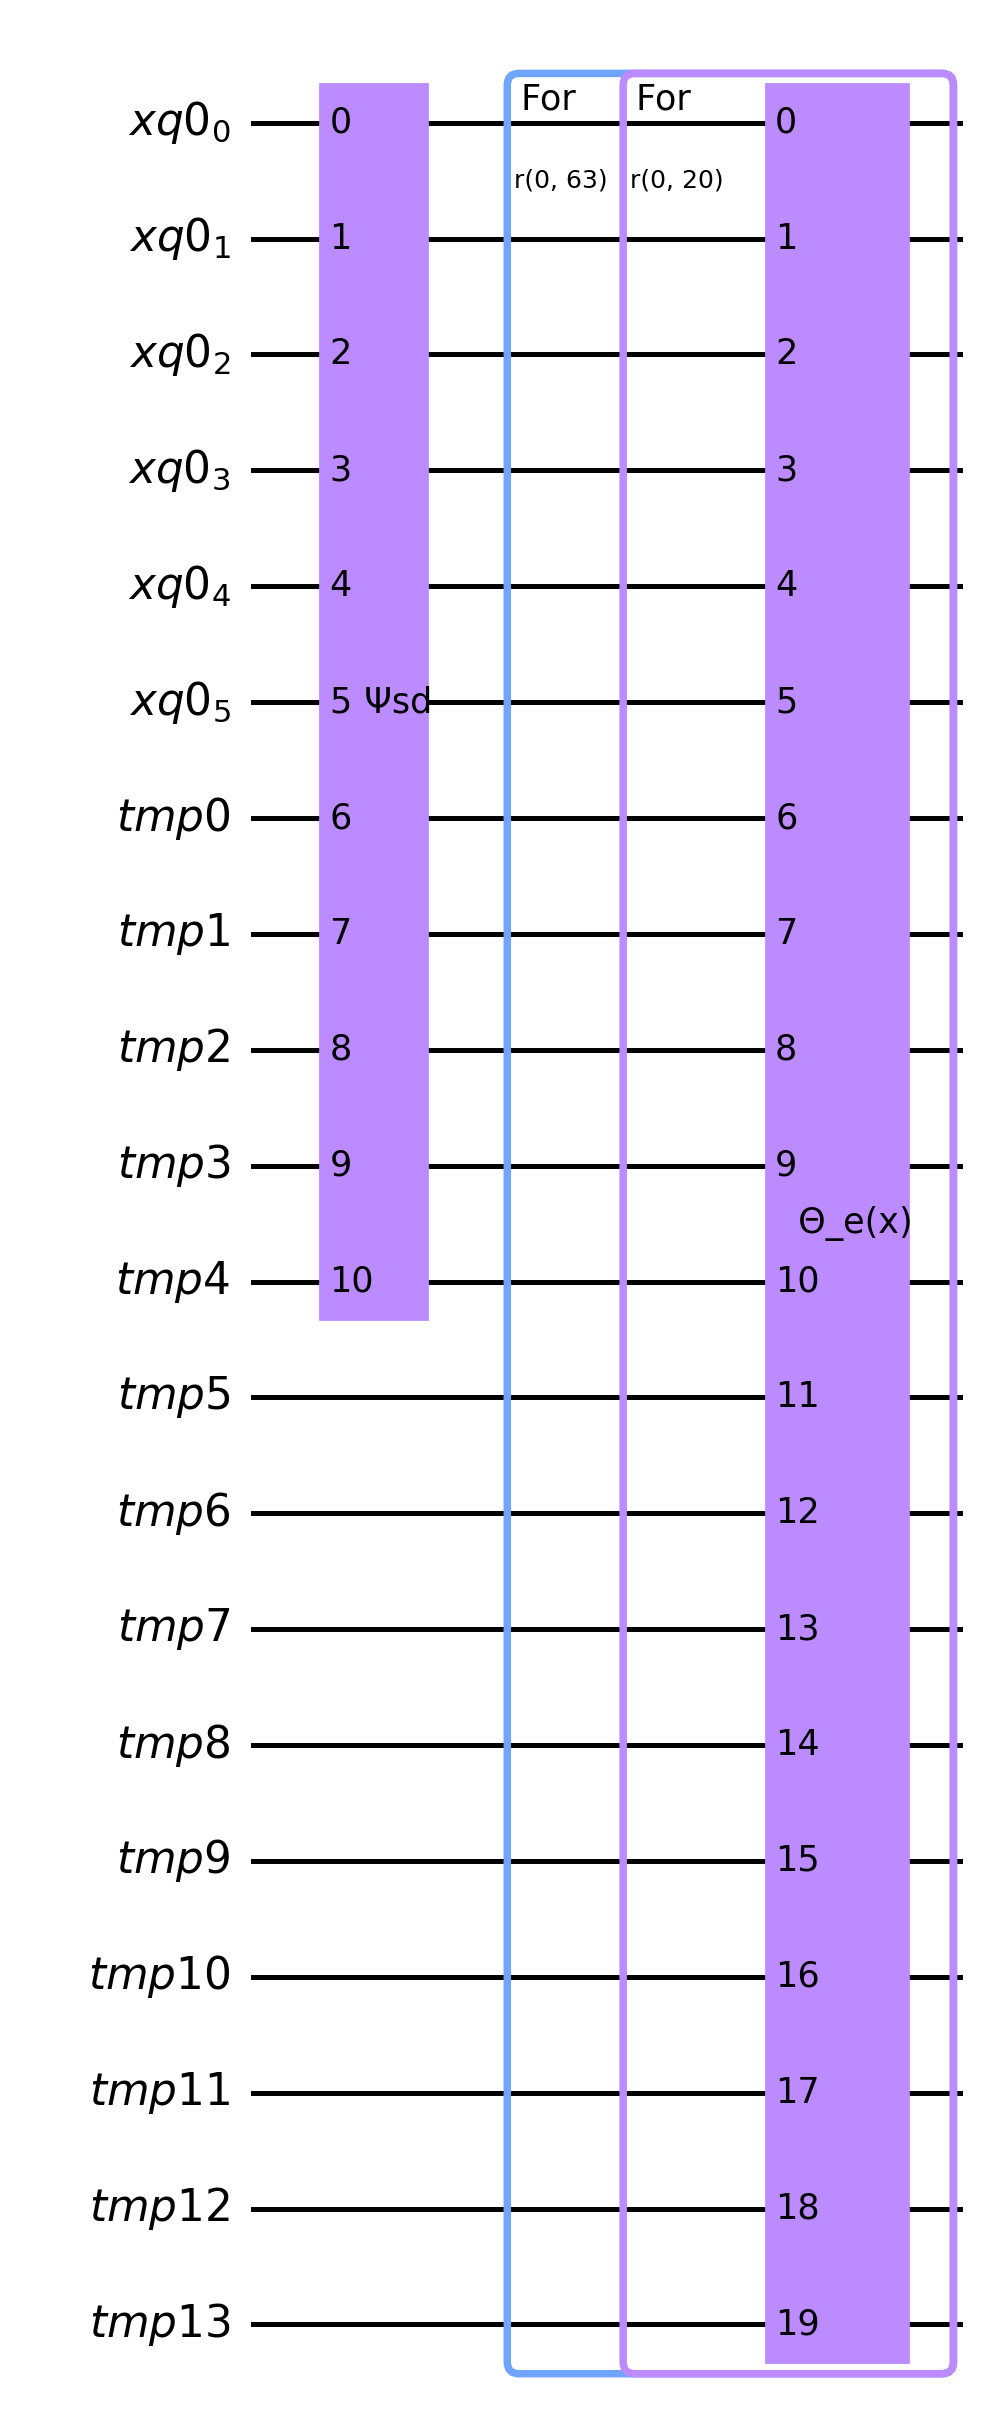
\includegraphics[width=\textwidth]{paper2025_figs/arith1D/circuit.png}
        \caption{回路の全体像}
        \label{subfig:circuit-1d-arith-overall}
    \end{subcaptionblock}
    \begin{subcaptionblock}[T][][t]{0.42\columnwidth}
        \centering
        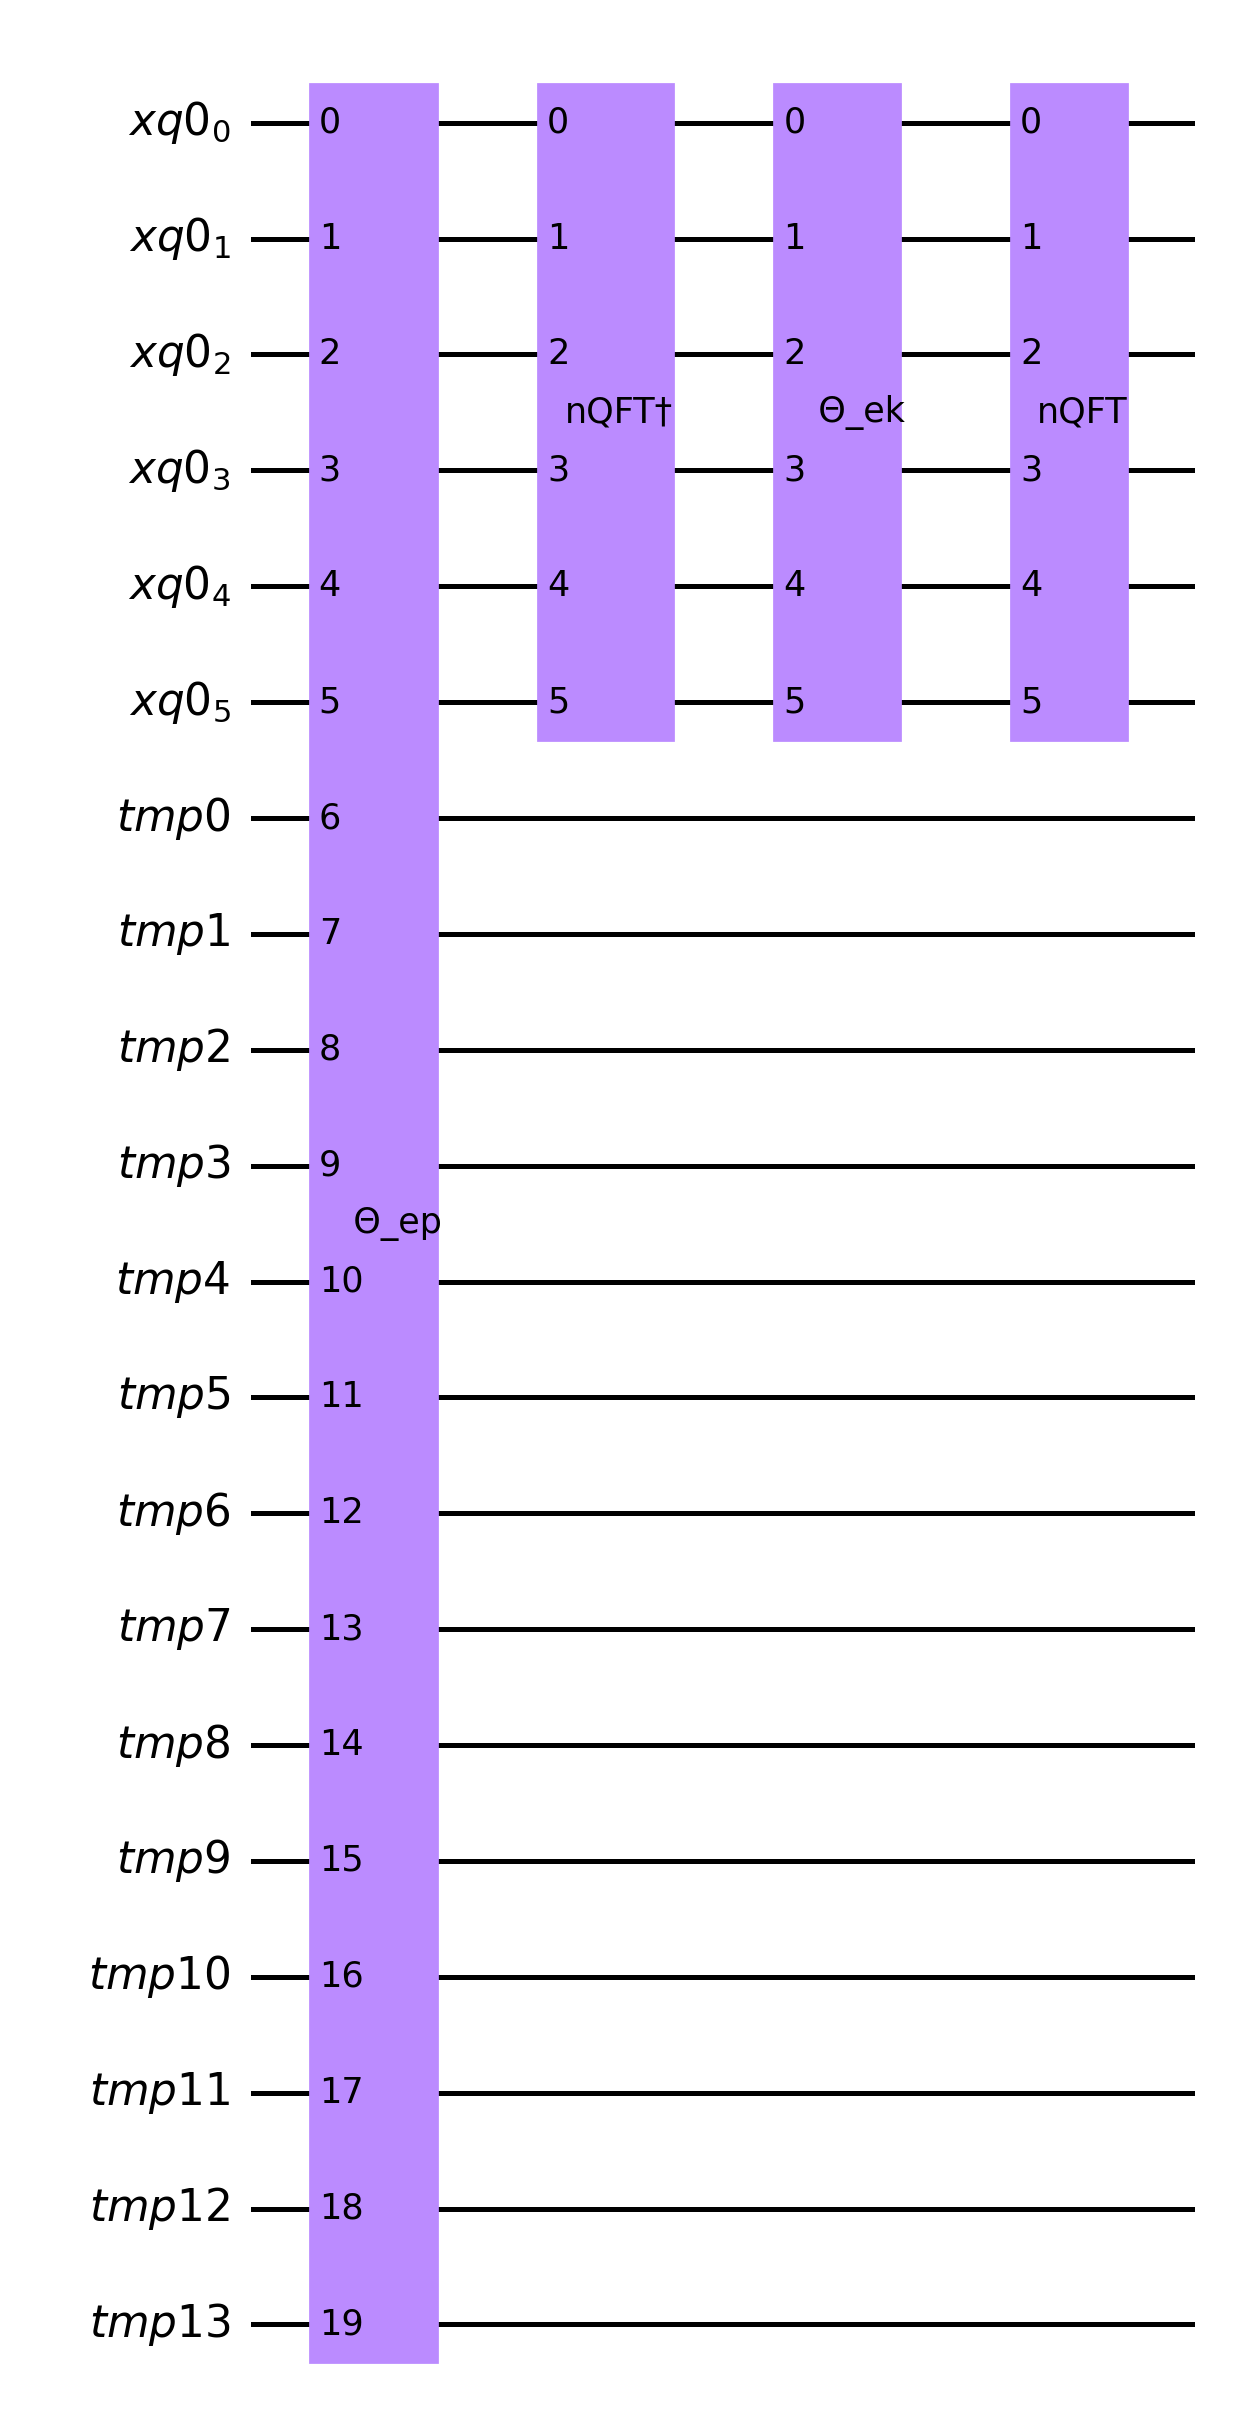
\includegraphics[width=\textwidth]{paper2025_figs/arith1D/elec_motion.png}
        \caption{時間発展回路$\Thetae$の内部}
        \label{subfig:circuit-1d-arith-time-evolution}
    \end{subcaptionblock}
    \caption{算術演算ゲートによる1次元モデルのシミュレータ回路}
    \label{fig:circuit-1d-arith}
    \begin{flushleft}\small
        (a) 1次元モデルのシミュレータ回路の全体像。初期化回路 $\PsiSD$ と時間発
        展回路 $\Thetae$ から構成される。(b) 時間発展回路 $\Thetae$ の内部構成。
        ポテンシャルエネルギー項回路 $\Thetaep$、逆QFT回路、運動エネルギー項回路
        $\Thetaek$、QFT回路からなる。$\Thetaep$ のqubit数（23ビット）が回路全体
        のqubit数を規定している。
    \end{flushleft}
\end{figure}

\begin{figure}[ht]
    \centering
    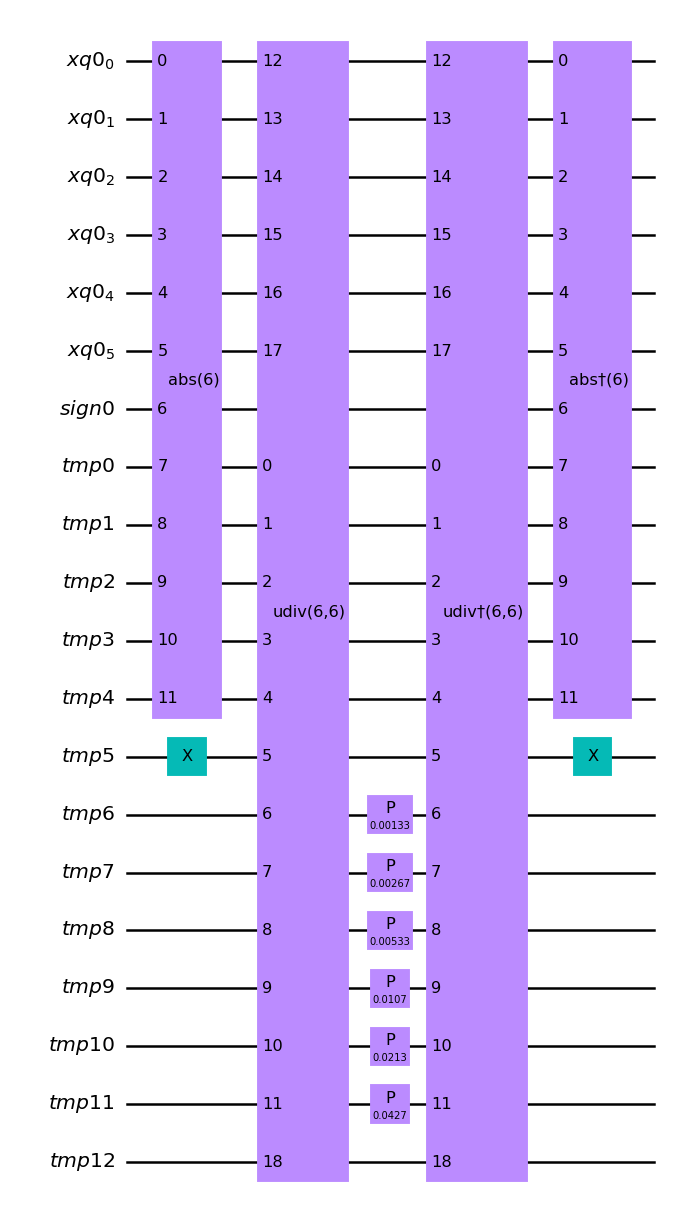
\includegraphics[width=0.5\textwidth]{paper2025_figs/arith1D/elec_potential_arithmetic.png}
    \caption{算術演算ゲートによるポテンシャルエネルギー項回路 $\Thetaep$}
    \label{subfig:potential-energy-circuit-1d-arith}
    \begin{flushleft}\small
        算術演算ゲートを用いて実装されたクーロンポテンシャル項回路 $\Thetaep$ の
        内部。算術演算で $1/|x|$ を2進数で計算し、結果のビット列の重みに応じてP
        ゲートで位相を変化させる。除算ゲート（udiv7）のqubit数が支配的であり、補
        助qubitの総数は17ビットである。
    \end{flushleft}
\end{figure}

\subsubsection{UCRZ回路を用いた回路構成}
\label{subsubsec:ucrz-circuit-configuration-results}
一方、クーロンポテンシャルの計算にUCRZ（Uniformly Controlled Rotation Z）回路を
用いた構成は、1次元および2次元モデルにおいてエミュレータの制限内に収まったが、3
次元モデルでは収まらなかった。

図\ref{fig:circuit-2d-ucrz}に、2次元水素原子モデルに対するUCRZ回路を用いたシミュ
レータの構成を示す。算術演算回路の場合とは異なり、ポテンシャル計算回路
$\Thetaepucr$ のqubit数は13ビットに抑えられており、回路全体のqubit数の決定要因で
はなくなっている。この構成においては、波動関数の状態準備回路 $\PsiSD$ が最も多く
のqubit数を要する。

\begin{figure}[ht]
    \centering
    \begin{subcaptionblock}[T][][t]{0.3\columnwidth}
        \centering
        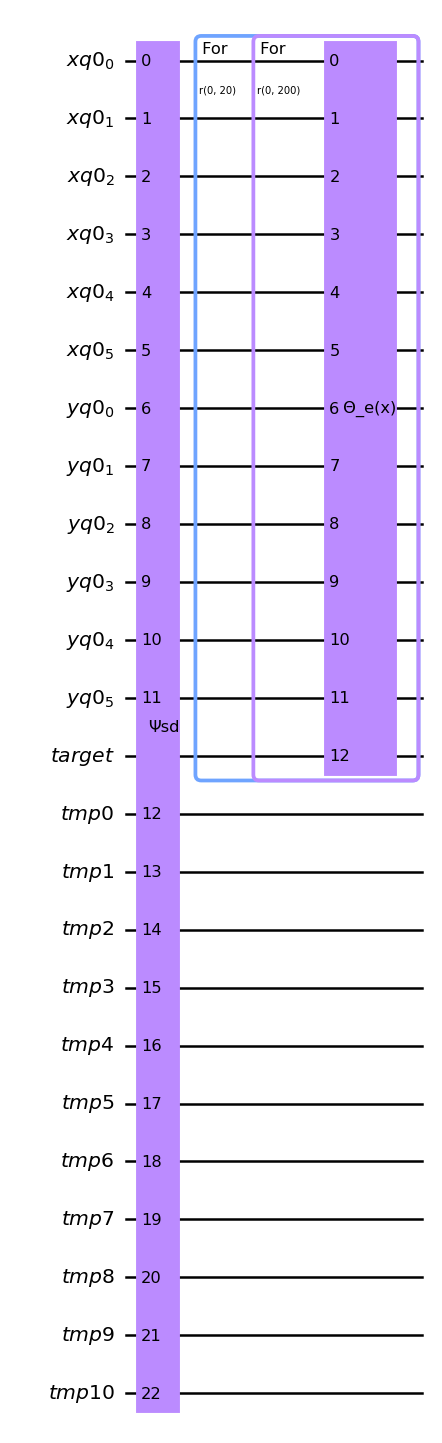
\includegraphics[width=\textwidth]{paper2025_figs/ucrz2D/circuit.png}
        \caption{シミュレータ全体}
        \label{subfig:circuit-2d-ucrz-overall}
    \end{subcaptionblock}
    \begin{subcaptionblock}[T][][t]{0.52\columnwidth}
        \centering
        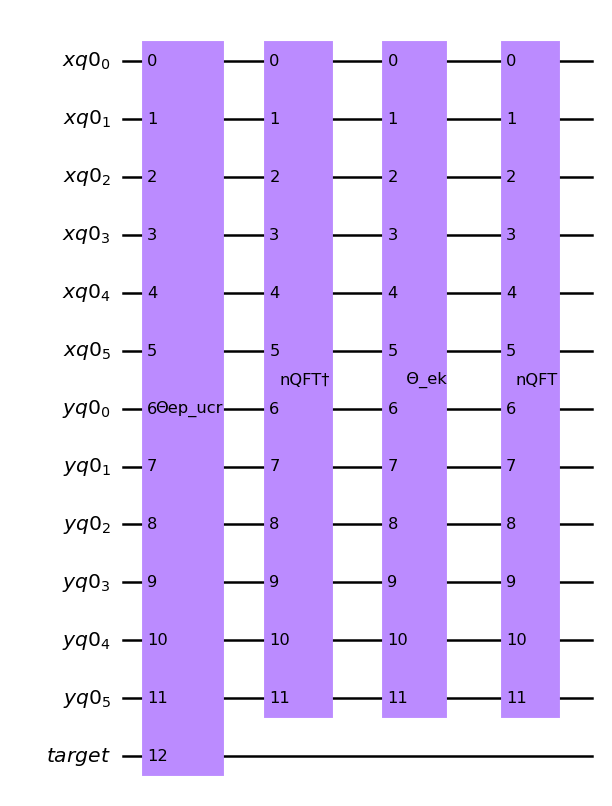
\includegraphics[width=0.8\textwidth]{paper2025_figs/ucrz2D/elec_motion.png}
        \caption{時間発展回路 $\Thetae$ の内部}
        \label{subfig:time-evolution-circuit-2d-ucrz}
    \end{subcaptionblock}
    \caption{UCRZ回路を用いた座標分解能6bit の2次元モデルのシミュレータ回路}
    \label{fig:circuit-2d-ucrz}
    \begin{flushleft}\small
        (a) シミュレータ回路の全体図。qubit数は状態準備回路の方が支配的であ
        る。(b) 時間発展回路の構成。ポテンシャルエネルギー項回路 $\Thetaepucr$
        はUCRZ回路を用いている。この例では入力レジスタ $xq0$, $yq0$（各6ビット、
        計12ビット）の値に応じて、唯一の補助qubitである $target$ の位相を変化さ
        せる。
    \end{flushleft}
\end{figure}

\clearpage
\subsubsection{回路規模の評価}
\label{subsec:circuit-size-evaluation-results}
本研究で使用した計算環境（エミュレータ）において、動作可能な現実的な上限はqubit
数が最大27、ゲート数が $10^7$ 程度である。この制約に対して、算術演算ゲート実装と
UCRZゲート実装のそれぞれで回路を生成し、次元数や座標分解能に対する回路規模
（qubit数およびゲート数）のスケーリングを評価した。

図\ref{fig:hamiltonian-gatecount}に、ポテンシャル回路 $\Thetaep$ の実装手法に応
じたqubit数と2量子ビットゲート数（時間発展1000ステップを想定）の比較を示す。
qubit数（上段）に関して、算術演算回路は1次元モデルでは絶対値計算で済むため少数の
qubitで実装可能だが、2次元・3次元モデルでは二乗および平方根を用いたノルム計算が
要求されるため回路が複雑化し、qubit数が激増する。結果として、算術演算回路がエ
ミュレータ制限（27 qubits）に収まるのは1次元の7ビット以下に限られる。対してUCRZ
回路は、3次元の8ビット分解能までqubit数の制限内に収まることが確認できた。

一方で、ゲート数（下段）に着目すると傾向が逆転する。算術演算回路のゲート数は次元
数が増えても緩やかにしか増加しないのに対し、UCRZ回路のゲート数は入力ビット数（次
元数 $\times$ 座標ビット数）に対して指数関数的に増大する性質を持つ。その結果、1
次元モデルや座標ビット数6ビット以下の2次元モデルではUCRZ回路の方がゲート数が少な
いが、3次元モデルにおいては全てのビット数において算術演算回路のゲート数がUCRZ回
路を下回る。

\begin{figure}[ht]
    \centering
    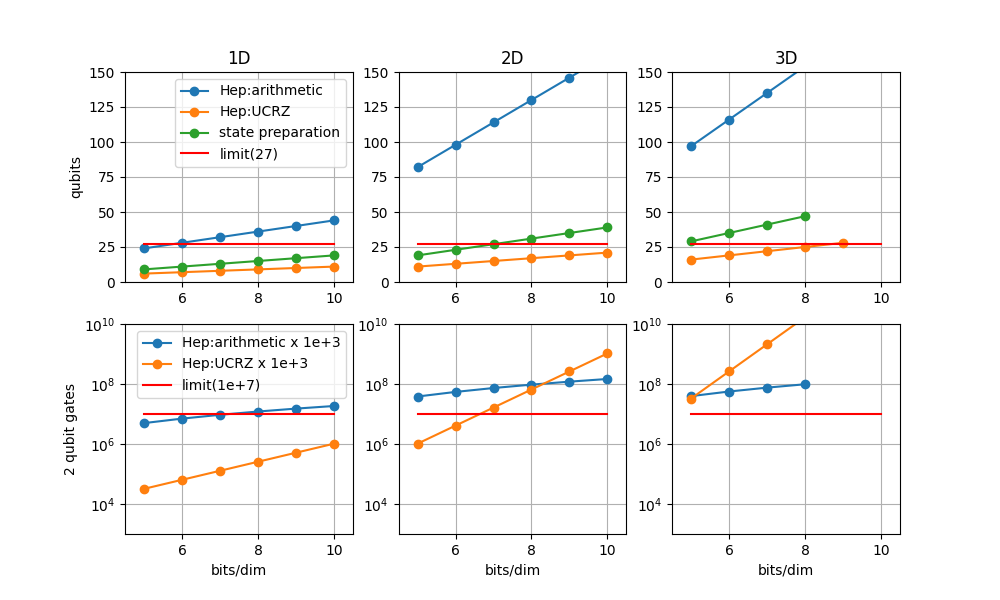
\includegraphics[width=15cm]{paper2025_figs/hamiltonian-gatecount.png}
    \caption{回路規模}
    \label{fig:hamiltonian-gatecount}
    \begin{flushleft}\small
    上段は1D〜3Dモデルにおける所要qubit数。算術演算回路は1D（7bit以下）でのみ制
    限（黒破線）に収まる一方、UCRZ回路は3D（8bit）まで制限内に収まる。2D/3Dでの
    算術演算回路のqubit数激増は、ノルム計算の複雑化に起因する。
    
    下段は1000ステップの時間発展に要する2量子ビットゲート数。算術演算回路は次元
    数に対する増加が緩やかだが、UCRZ回路は入力ビット数に対して指数的に増加するた
    め、3D環境下では算術演算回路の方がゲート数の観点から有利となる。
    \end{flushleft}
\end{figure}

これらの評価から、実際に量子コンピュータ（またはエミュレータ）で回路を動作させる
場合、対象とするモデルの次元数と利用可能なqubit数・ゲート数（コヒーレンス時間）
のトレードオフを考慮し、最適な実装方式を選択する必要があることが示された。本エ
ミュレータ環境下で実際に動作可能であった回路構成の組み合わせを表
\ref{tab:emulator-circuit-configurations}にまとめる。

\begin{table}[ht]
\centering
\caption{エミュレータで動作した回路構成一覧}
\begin{tabular}{rcc}
    \hline
    次元数 & 算術ゲート版回路の$\nb$ & UCRZ版回路の$\nb$ \\
    \hline
    1 & 6,7 & 評価せず（算術演算で動作したため） \\
    2 & 動作せず & 6 \\
    3 & 動作せず & 動作せず \\
    \hline
\end{tabular}
\label{tab:emulator-circuit-configurations}
\end{table}

表\ref{tab:emulator-circuit-configurations}の条件において、第
\ref{sec:coulomb-potential-handling}節で定式化したクーロンポテンシャルの特異点処
理を適用し、第\ref{sec:parameter-selection-for-minimum-error}節で導出した最適シ
ミュレーションパラメータを設定することで、算術演算回路・UCRZ回路のいずれを用いて
も期待通りの波動関数の時間発展が確認できた。得られた計算誤差の詳細な分析について
は、次項以降で述べる。

\begin{figure}[ht]
    \centering
    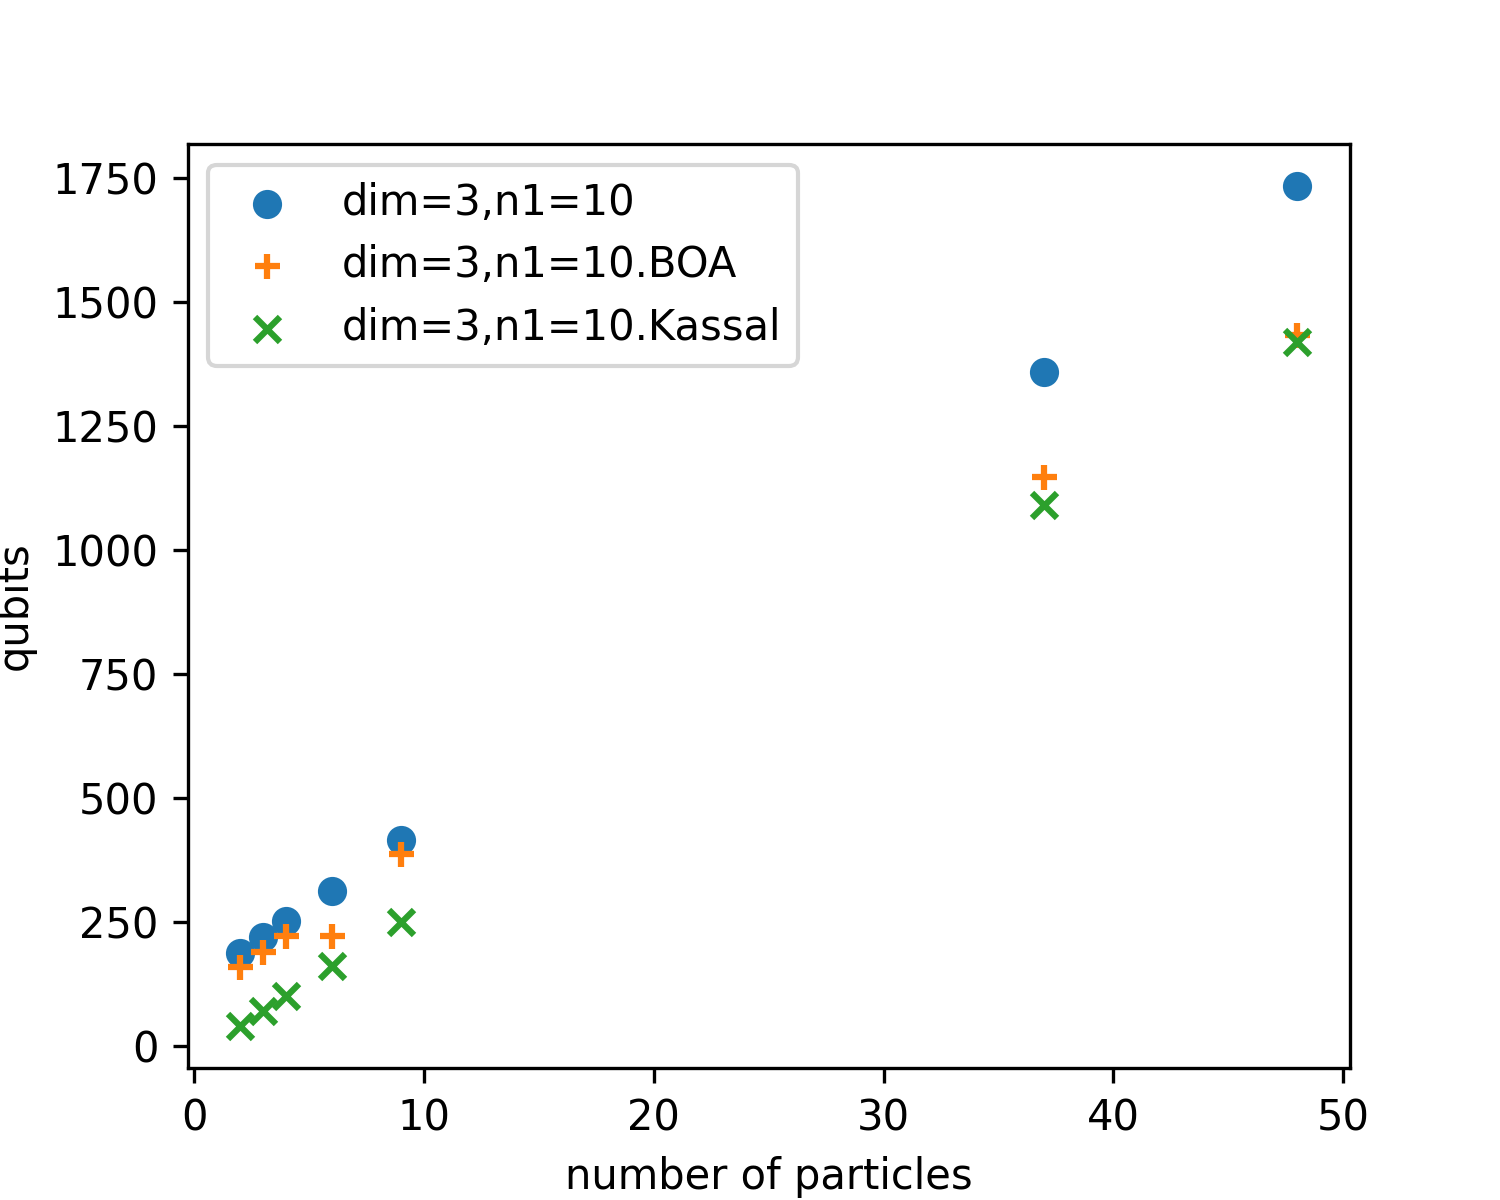
\includegraphics[width=0.6\textwidth]{paper2025_figs/circuit-size-qubits.png}
    \caption{粒子数とqubit数の関係}
    \label{fig:qubit-for-some-molecules}
    \begin{flushleft}\small

        横軸は粒子数（電子数＋原子核数）、縦軸は算術演算回路（3次元、座標10ビッ
        ト）を用いた場合の所要qubit数。各点は左から \ce{H}, \ce{He}, \ce{Li},
        \ce{H + H2}, \ce{O}, Glycine(\ce{C2H5NO2}), Alanine(\ce{C3H7NO2}) を示
        す。「\verb|+|」は原子核位置を固定した場合（Born-Oppenheimer近
        似）。「\verb|x|」はKassalら\cite{kassal2008.pnas.0808245105}の見積もり
        式に基づく値。
    \end{flushleft}
\end{figure}

最後に、将来的な大規模量子コンピュータでの実行を見据え、エミュレータの制限を度外
視して様々な原子・分子モデルに対して本提案の算術演算回路（3次元、分解能10ビッ
ト）を生成し、スケーラビリティを評価した。図\ref{fig:qubit-for-some-molecules}に
示す通り、必要となるqubit数は系の粒子数（電子数と原子核数の和）に対して線形にス
ケーリングすることが確認できる。

\subsection{クーロンポテンシャルの極の扱い}
\label{subsec:coulomb-potential-handling-results}
本項では、第\ref{sec:coulomb-potential-handling}節で定式化したクーロンポテンシャ
ルの特異点（極）における発散回避手法について、局所平均ポテンシャルとSoft-coreポ
テンシャルのそれぞれを用いた場合のエネルギー評価結果を示す。

\subsubsection{局所平均ポテンシャルを用いる方法}
\label{subsubsec:local-average-potential-results}

式\eqref{eq:Halr}で定義した局所平均ポテンシャル $\Hla(r)$ において、実効半径を
$\reff = \deltar/a$ と置き、係数 $a$ を $1 \le a \le 8$ の範囲で変化させたときの
エネルギー計算値を複数のqubit数 $\nb$ に対して評価した。なお、本評価にはエミュ
レータの制限（qubit数上限）を超えるパラメータが含まれるため、量子回路の動作と等
価な演算を行う古典シミュレーションプログラムを用いて計算を実施した。

2次元モデルの波動関数 $\PsiTwoD_{0,0}$ および $\PsiTwoD_{1,0}$ に対する評価結果
をそれぞれ図\ref{fig:Ha1-vs-delta1}の(a)および(b)に示す。グラフから明らかなよう
に、両方の状態において $a=4$、すなわち $\reff = \deltar/4$ と設定した際に、エネ
ルギー期待値が解析解（それぞれ $-2.0\ \mathrm{a.u.}$、$-0.2222\ \mathrm{a.u.}$）
に最もよく一致する結果が得られた。

どの分解能（ビット数）においても $a=4$ を境に誤差の符号が反転しており、最適条件
がビット数に依存せず共通していることが確認できる。これは、微小領域における積分値
の整合性から $\reff \approx \deltar/4$ を導出した第
\ref{sec:coulomb-potential-handling}節の理論的近似が妥当であることを強く裏付けて
いる。

\begin{figure}[ht]
    \centering
    \begin{subfigure}{0.45\columnwidth}
        \centering
        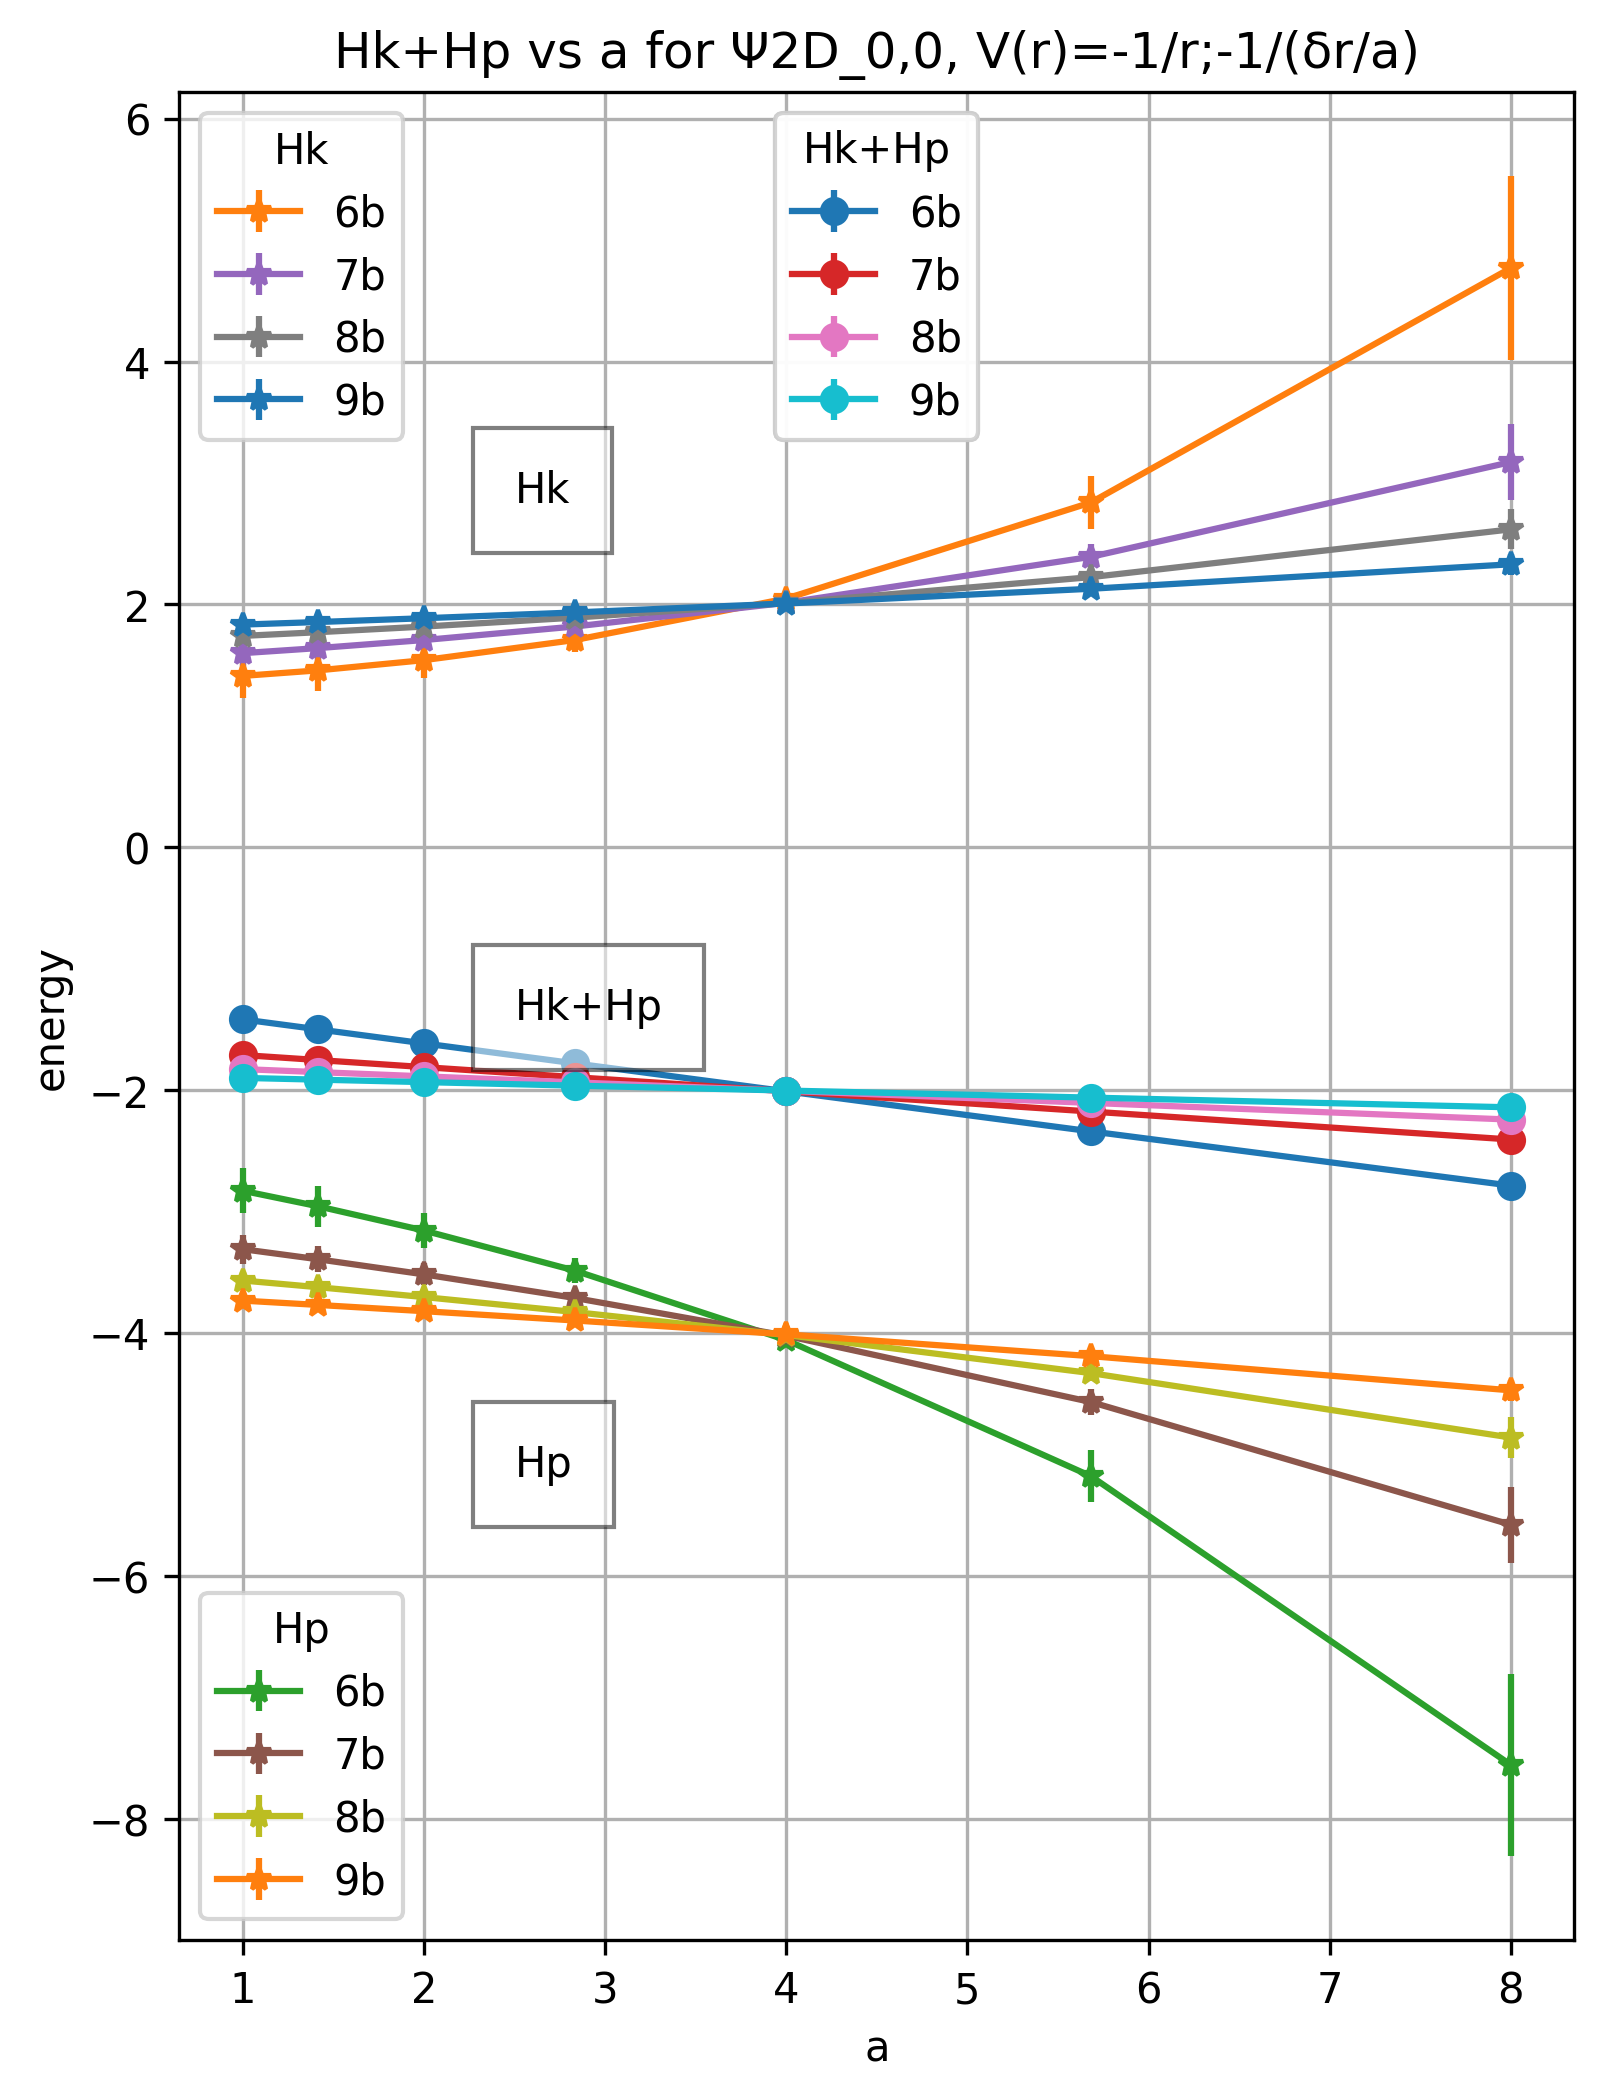
\includegraphics[width=1\columnwidth]{paper2025_figs/compare_energy/compare_energy_h2D_TO2_r0lim_0_0.png}
        \caption{$\PsiTwoD_{0,0}$}
        \label{subfig:Ha1-energy-0-0}
    \end{subfigure}
    \begin{subfigure}{0.47\columnwidth}
        \centering
        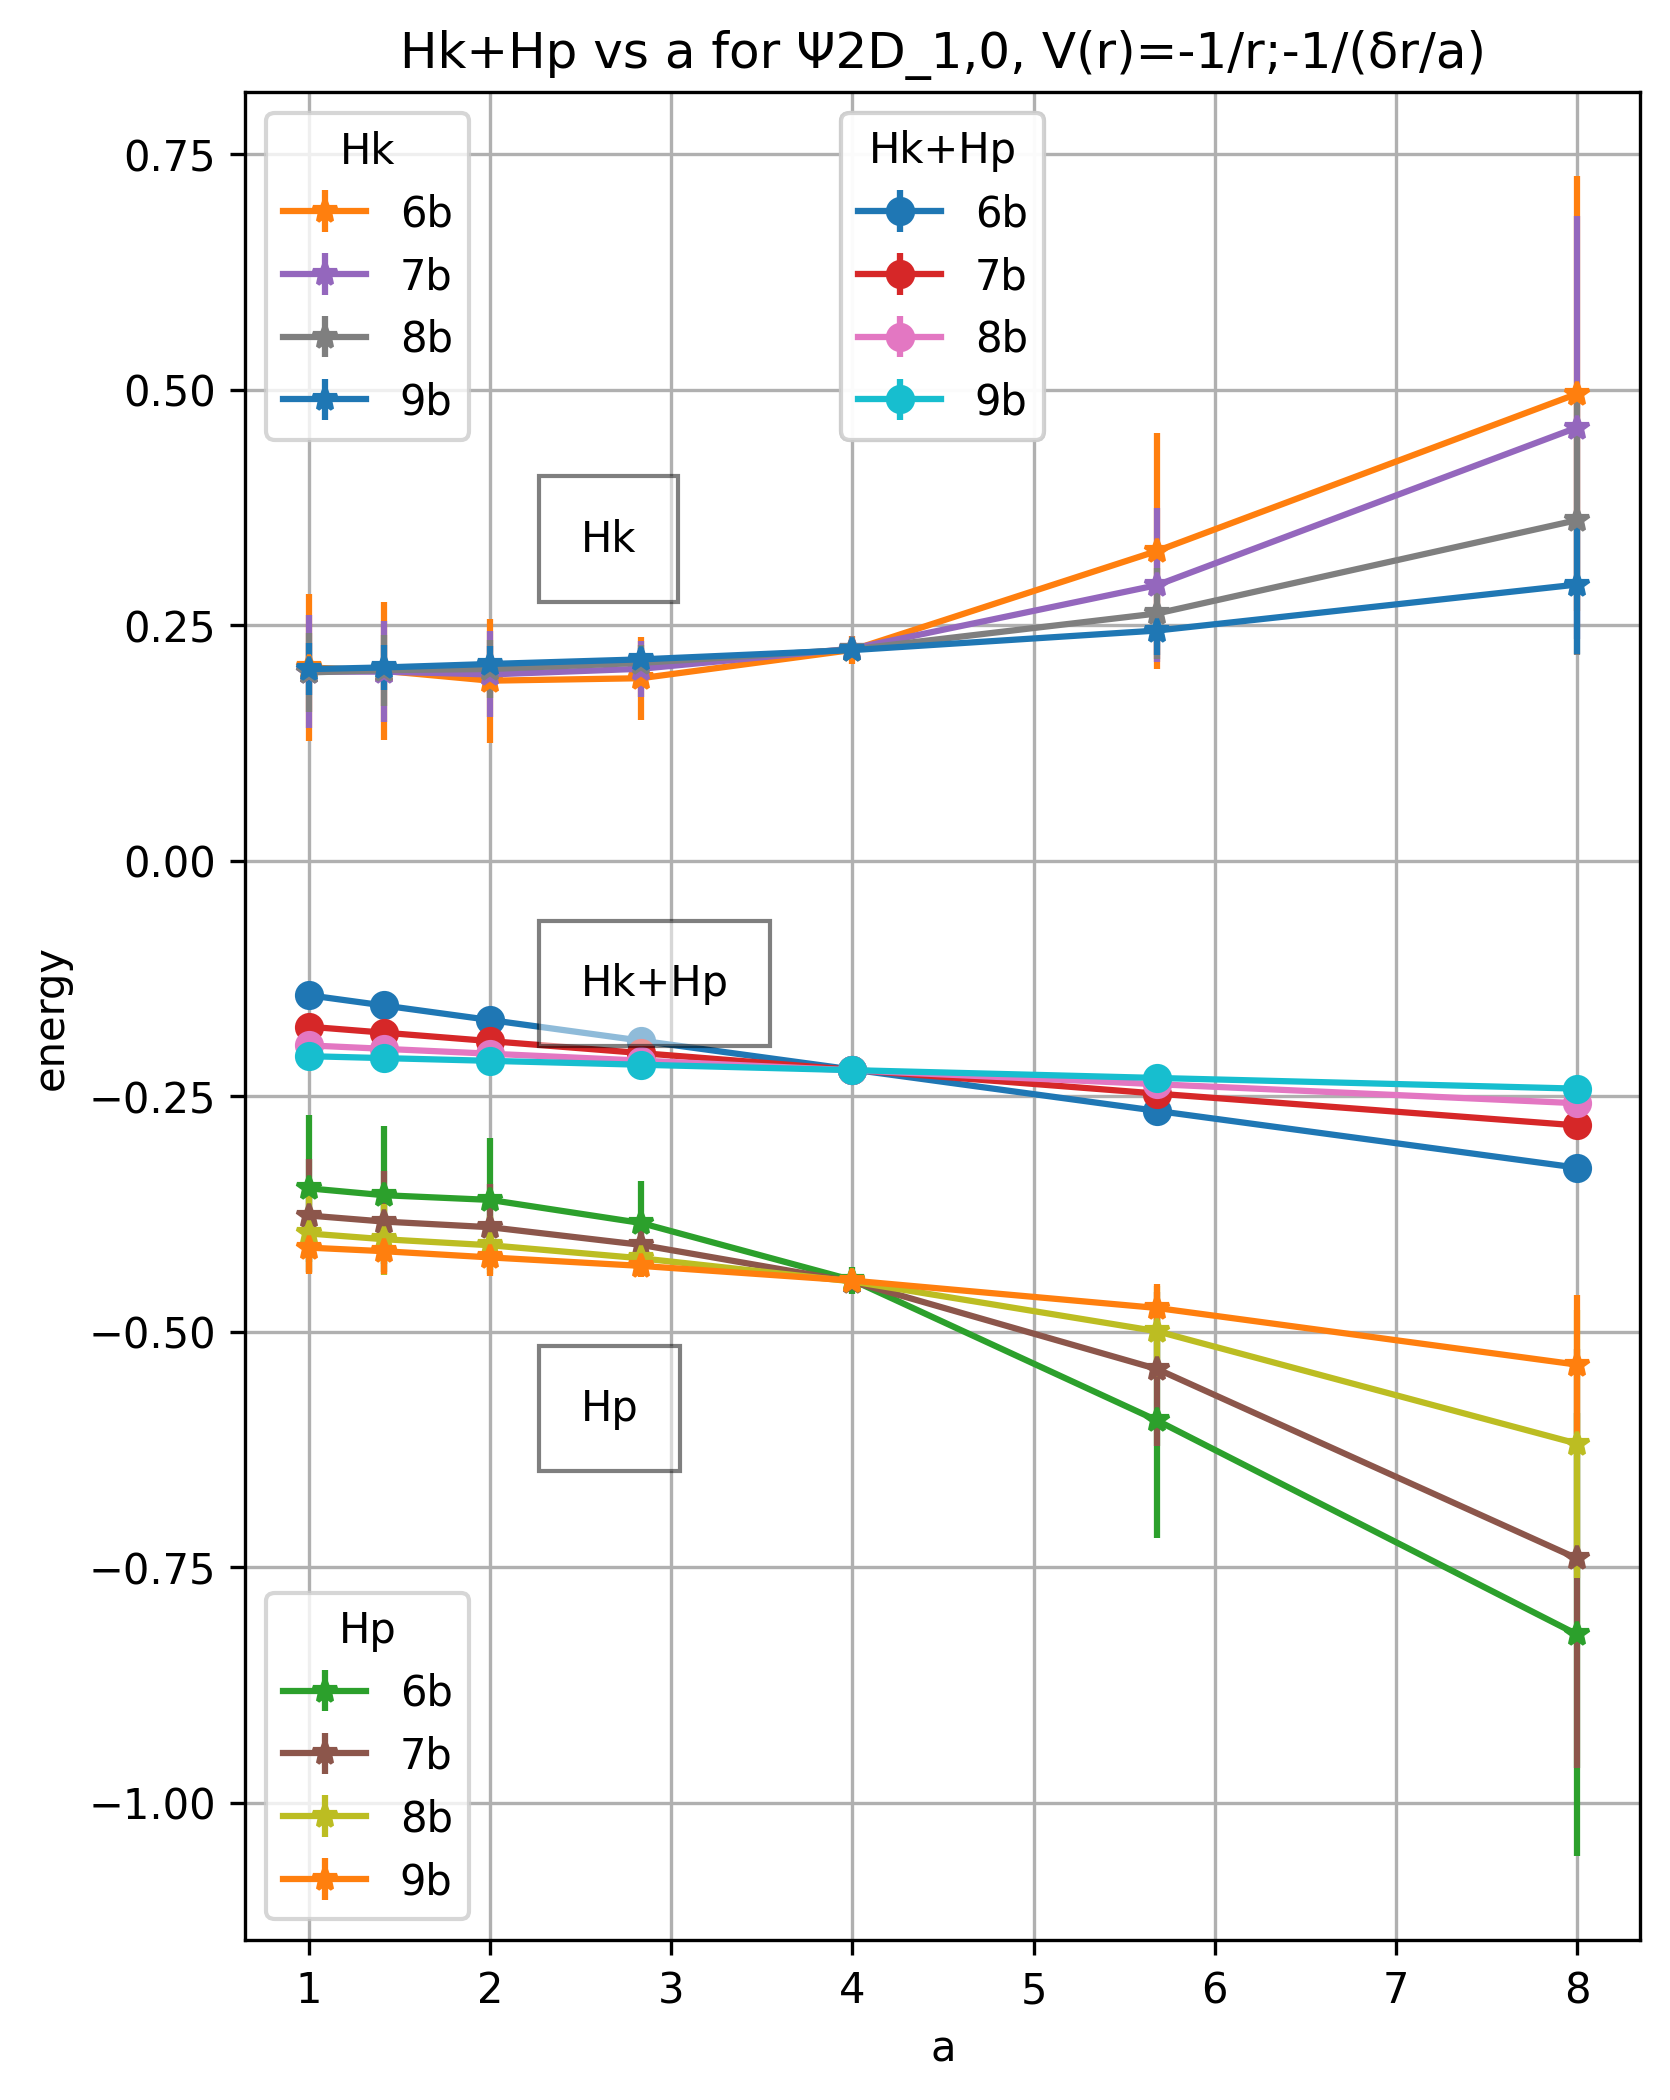
\includegraphics[width=1\columnwidth]{paper2025_figs/compare_energy/compare_energy_h2D_TO2_r0lim_1_0.png}
        \caption{$\PsiTwoD_{1,0}$}
        \label{subfig:Ha1-energy-1-0}
    \end{subfigure}
    \caption{近似式$\Hla(r)$において$\reff$の値を変えた時のエネルギー値の変化}
    \label{fig:Ha1-vs-delta1}
    \begin{flushleft}\small
        (a) 状態 $\PsiTwoD_{0,0}$ に対して $\reff=\deltar/a$ と置き、$a$ を変化
        させたグラフ。横軸の $a$ は比が $\sqrt{2}$ の等比数列としている。全ての
        ビット数において、$a=4$（$\reff=\deltar/4$）の時にハミルトニアンの期待値
        $\Hk+\Hp$ が解析解である $-2.0$ に肉薄している。 (b) 状態
        $\PsiTwoD_{1,0}$ に対する結果。同様に $a=4$ において解析解 $-0.2222$ に
        最も近い値を示している。
    \end{flushleft}
\end{figure}

\subsubsection{ソフトコアポテンシャル}
\label{subsubsec:soft-core-potential-results}
次に、式\eqref{eq:Hsc2r}で定義したSoft-coreポテンシャル $\Hsc(r)$ について、オフ
セット定数を $\Delta = \deltar/a$ と置いて $a$ を変化させたときのエネルギー計算
値を図\ref{fig:Ha2-vs-delta2}に示す（計算手法は前項と同様である）。

Soft-coreポテンシャルは特異点 $r=0$ において $\Hsc(0)=-1/\Delta$ となり、局所平
均ポテンシャル $\Hla(0)=-1/\reff$ と全く同じ定数形態をとる。図
\ref{fig:Ha2-vs-delta2}の結果からも読み取れるように、$\Hla(r)$ の場合と同様に
$a=4$（すなわち $\Delta=\deltar/4$）を採用した際に、エネルギー期待値が解析解に最
も近い値を示した。

$r \neq 0$ の領域では両者の関数形に差異があるものの、エネルギー期待値の誤差を支
配しているのは特異点近傍での振る舞いであるため、結果的に全体の計算値には大きな差
が生じなかったと考えられる。この結果は、Soft-coreポテンシャルを特異点の正則化目
的で使用する場合にも、局所平均ポテンシャルから導出された $\Delta = \deltar/4$ と
いう境界条件が最適パラメータとして機能することを示している。

\begin{figure}[ht]
    \centering
    \begin{subfigure}{0.45\columnwidth}
        \centering
        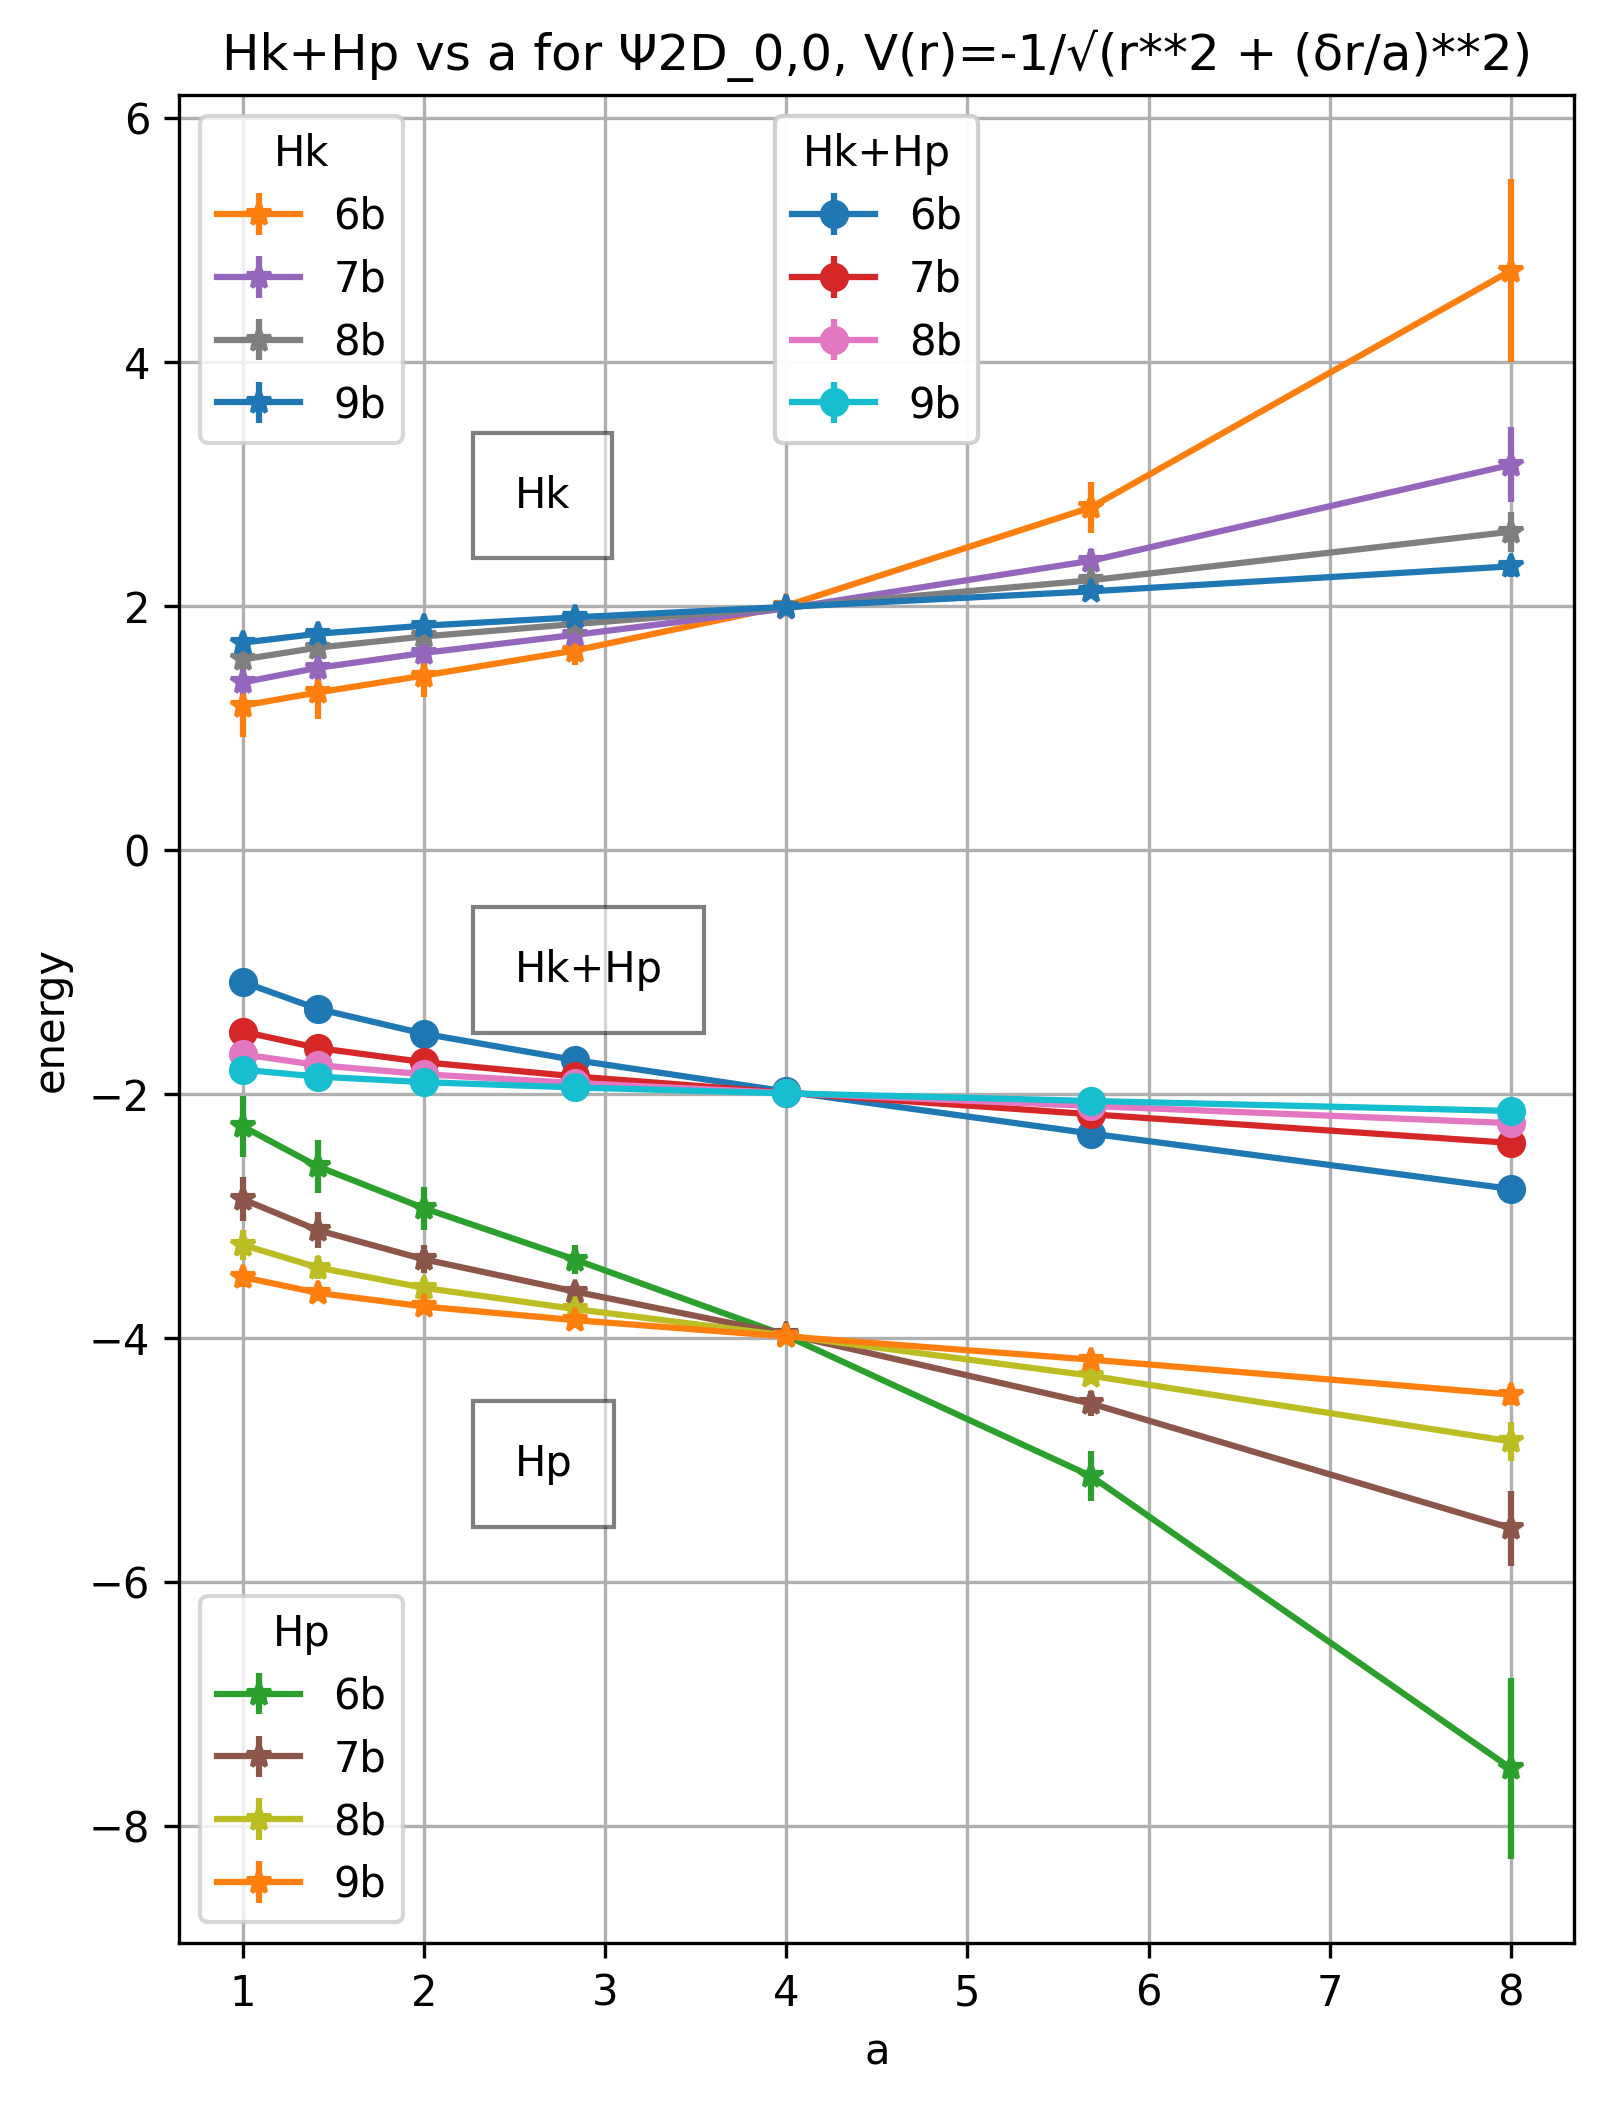
\includegraphics[width=1\columnwidth]{paper2025_figs/compare_energy/compare_energy_h2D_TO2_rofs_0_0.png}
        \caption{$\PsiTwoD_{0,0}$}
        \label{subfig:Ha2-energy-0-0}
    \end{subfigure}
    \begin{subfigure}{0.47\columnwidth}
        \centering
        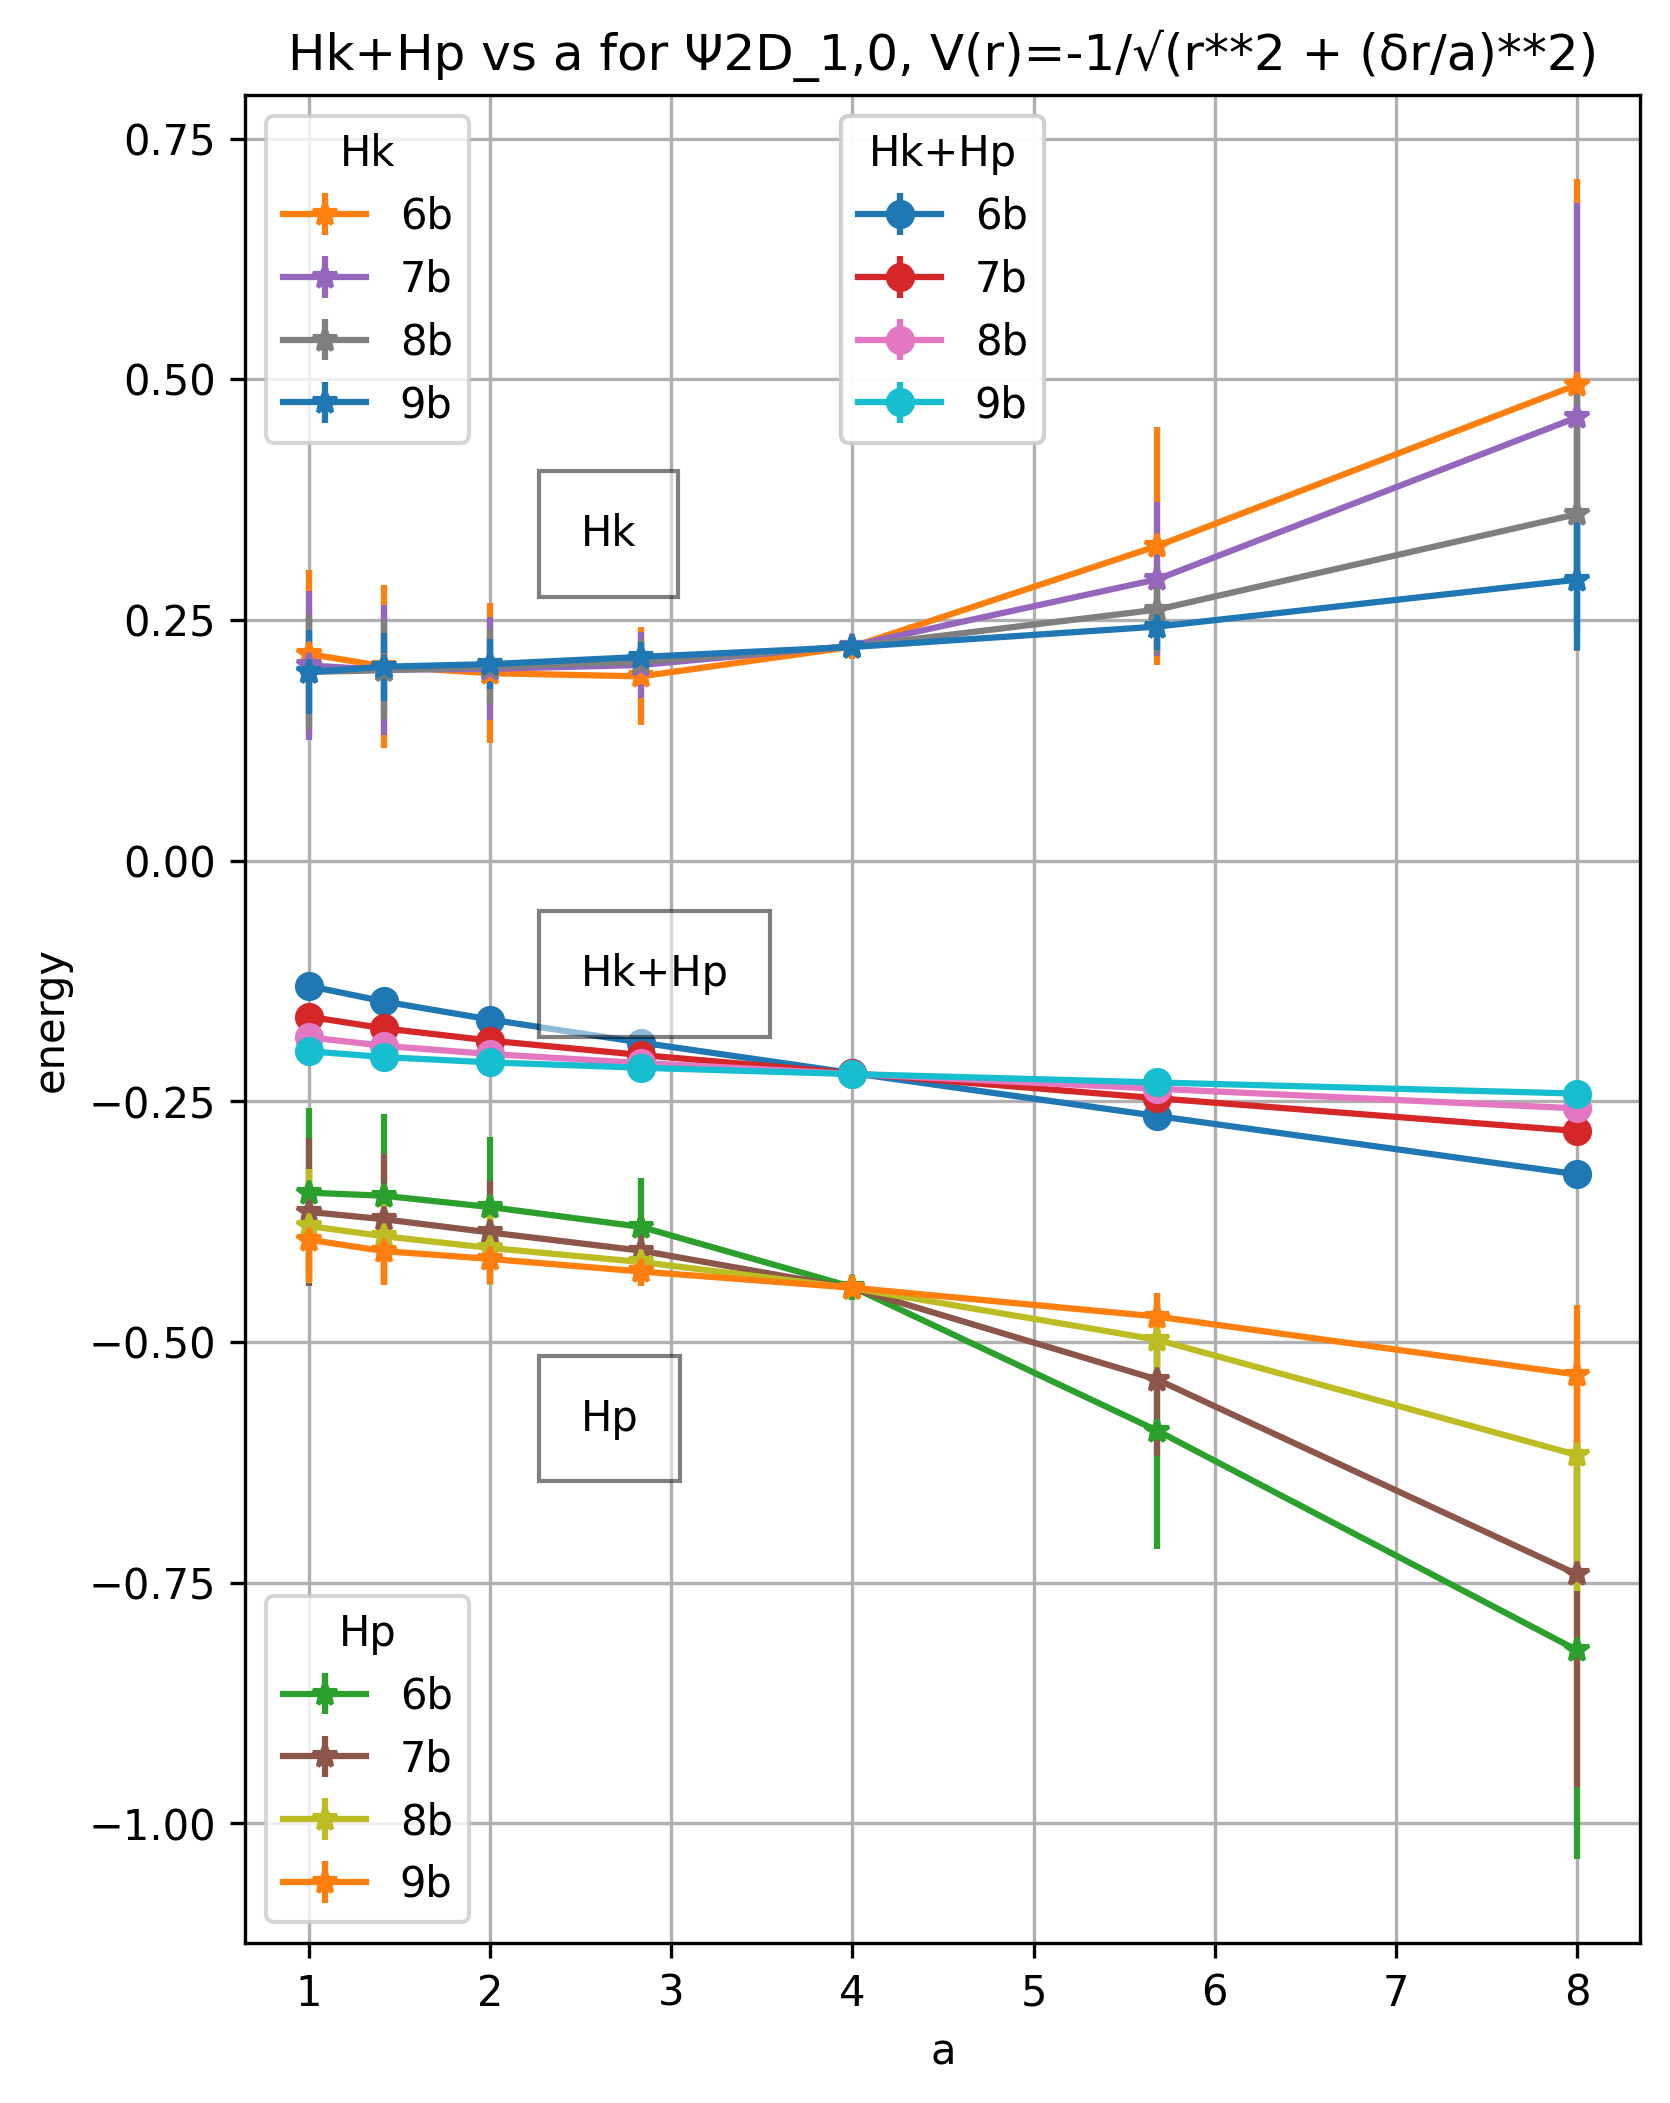
\includegraphics[width=1\columnwidth]{paper2025_figs/compare_energy/compare_energy_h2D_TO2_rofs_1_0.png}
        \caption{$\PsiTwoD_{1,0}$}
        \label{subfig:Ha2-energy-1-0}
    \end{subfigure}
    \caption{近似式$\Hsc(r)$において$\Delta$の値を変えた時のエネルギー値の変化}
    \label{fig:Ha2-vs-delta2}
    \begin{flushleft}\small
        (a) 状態 $\PsiTwoD_{0,0}$ に対して $\Delta=\deltar/a$ と置き、$a$ を変化
        させたグラフ（$a$ は比が $\sqrt{2}$ の等比数列）。全てのビット数において
        $a=4$（$\Delta=\deltar/4$）の時に $\Hk+\Hp$ が解析解 $-2.0$ に最も近い値
        を示している。 (b) 状態 $\PsiTwoD_{1,0}$ に対する結果。同様に $a=4$ にお
        いてエネルギー期待値が解析解 $-0.2222$ に最も近い。
    \end{flushleft}
\end{figure}
\clearpage

\subsection{誤差を最小にするシミュレーションパラメータ}
\label{subsec:parameter-selection-for-minimum-error-results}
本項では、第\ref{sec:parameter-selection-for-minimum-error}節で論じた誤差最小化
のためのパラメータ決定手法について、具体的な数値評価の結果を示す。まず、空間離散
化誤差とカットオフ誤差のトレードオフに基づく格子間隔の最適化について述べ、続いて
サンプリング定理およびSuzuki-Trotter分解に基づく時間パラメータ（分割数）の評価結
果を示す。

\subsubsection{格子間隔の決定方法}
\label{subsubsec:delta-r-selection-results}

図\ref{fig:dq-tradeoff}の(a)に、1次元モデルの波動関数 $\PsiOneD_1$ を対象とし
て、複数のqubit数 $\nb$ における空間離散化誤差 $\errdisc = |S_d-S_1|$ とカットオフ誤
差 $\errcutoff = S_2$ の関係を評価した結果を示す。

qubit数が最も少ない $\nb=6$ のケースに着目すると、(A2)のグラフにおいて
$\errcutoff$ と $\errdisc$ の曲線が $\deltar \approx 0.22$ 付近で交差している。
この点が二つの誤差のトレードオフが均衡する値であり、両者の和である(A3)のグラフが
最小値を取る最適パラメータに該当する。このとき、シミュレーション領域の寸法は
$L=14$ となる。((A1)には、波動関数の振幅実部と $\pm L/2$ の境界位置を垂直線で示
している。)

一方、qubit数を増やした $\nb=8$ のケースでは、(A3)のグラフから誤差の和が最小（ほ
ぼゼロ）となる $\deltar$ の範囲が $0.07 \sim 0.14$ と広く平坦になっていることが
分かる。これは、qubit数という計算リソースに余裕がある条件下では、最適パラメータ
の選択幅が広がることを意味する。なお、この範囲を外れて $\deltar < 0.07$ で誤差が
急増するのは空間サイズ $L$ の縮小によるカットオフ誤差の顕在化に起因し、逆に
$\deltar > 0.14$ で誤差が増加するのは空間分解能の粗さによる空間離散化誤差の増大に起
因する。

図\ref{fig:dq-tradeoff}の(b)および(c)に、2次元モデルの波動関数 $\PsiTwoD_{0,0}$
と $\PsiTwoD_{1,0}$ に対する結果をそれぞれ示す。対象とする状態（波動関数の空間的
な広がり）の違いに応じて、適切な $\deltar$ の最適範囲が大きく変化することが確認
できる。

\begin{figure}[ht]
    \centering
    \begin{subfigure}{1.0\columnwidth}
        \centering
        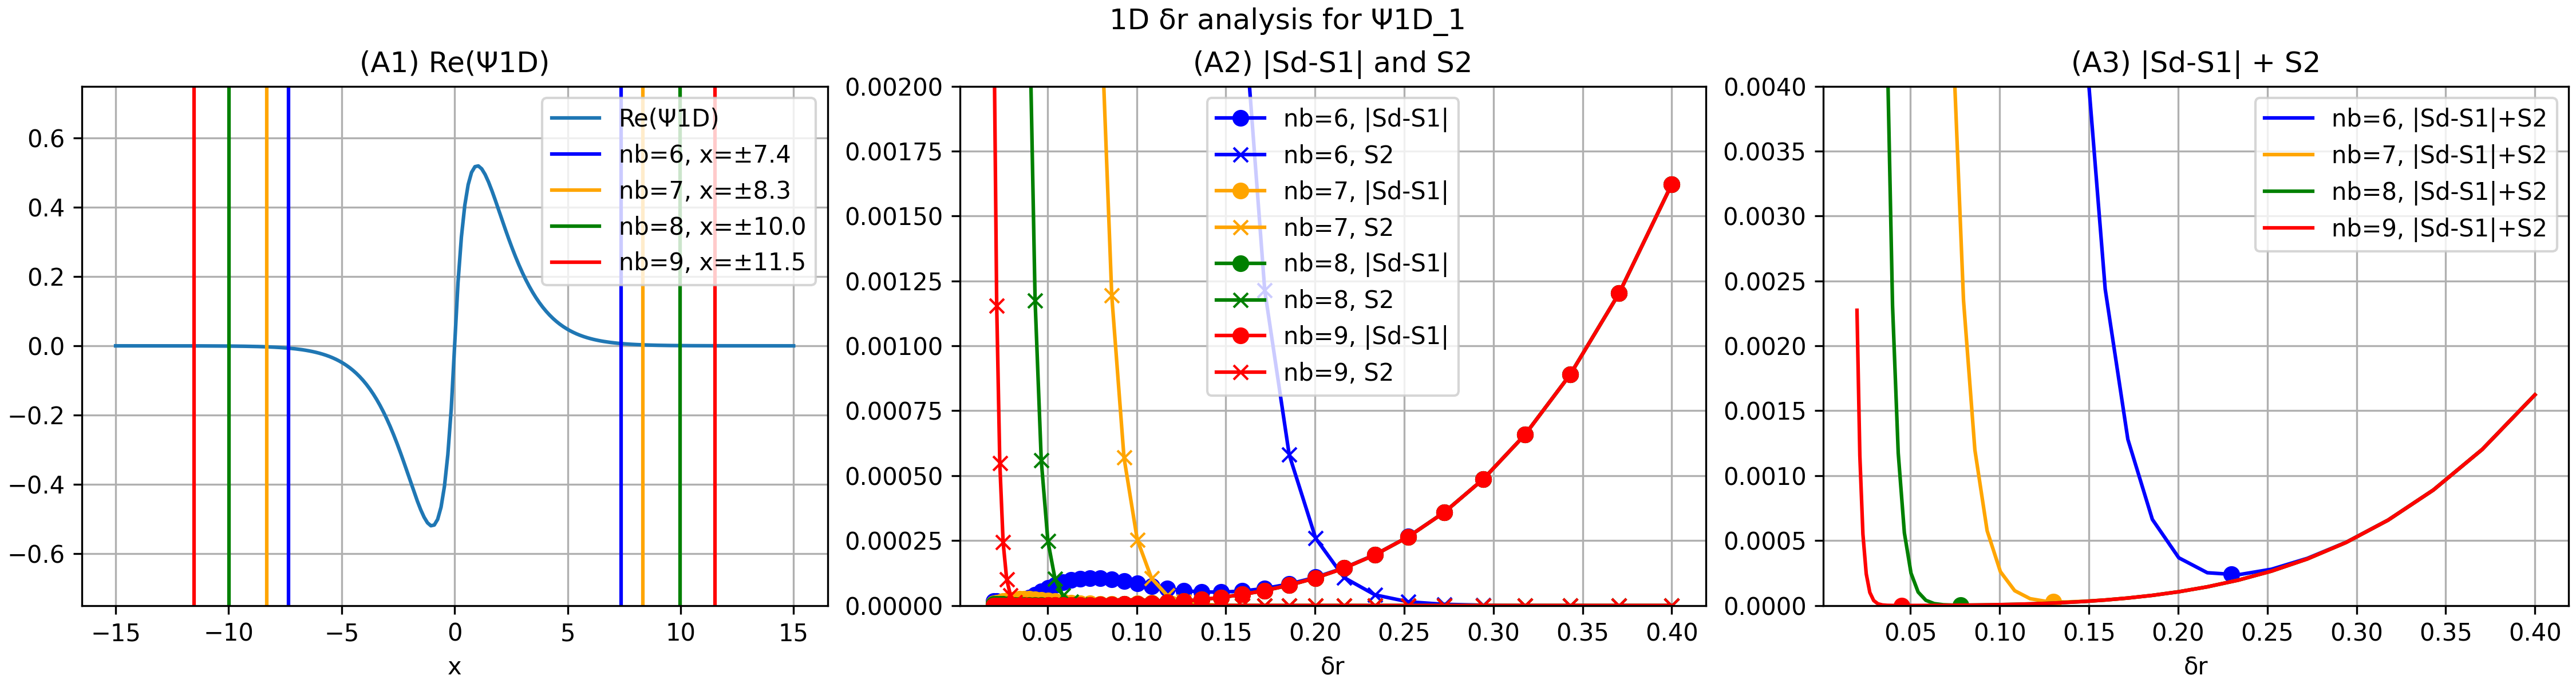
\includegraphics[width=\columnwidth]{paper2025_figs/dq_tradeoff/eval1d_dq.png}
        \caption{1次元モデル $\PsiOneD_1$}
        \label{subfig:dq-tradeoff-1d}
    \end{subfigure}
    \begin{subfigure}{1.0\columnwidth}
        \centering
        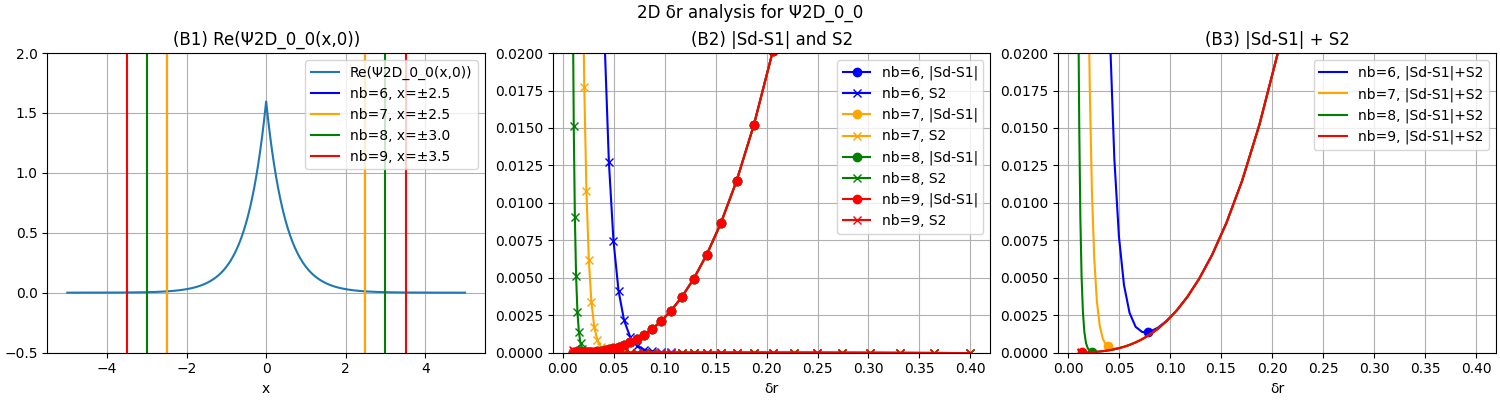
\includegraphics[width=\columnwidth]{paper2025_figs/dq_tradeoff/eval2d_dq_geom_0_0.png}
        \caption{2次元モデル $\PsiTwoD_{0,0}$}
        \label{subfig:dq-tradeoff-2d-0-0}
    \end{subfigure}
    \begin{subfigure}{1.0\columnwidth}
        \centering
        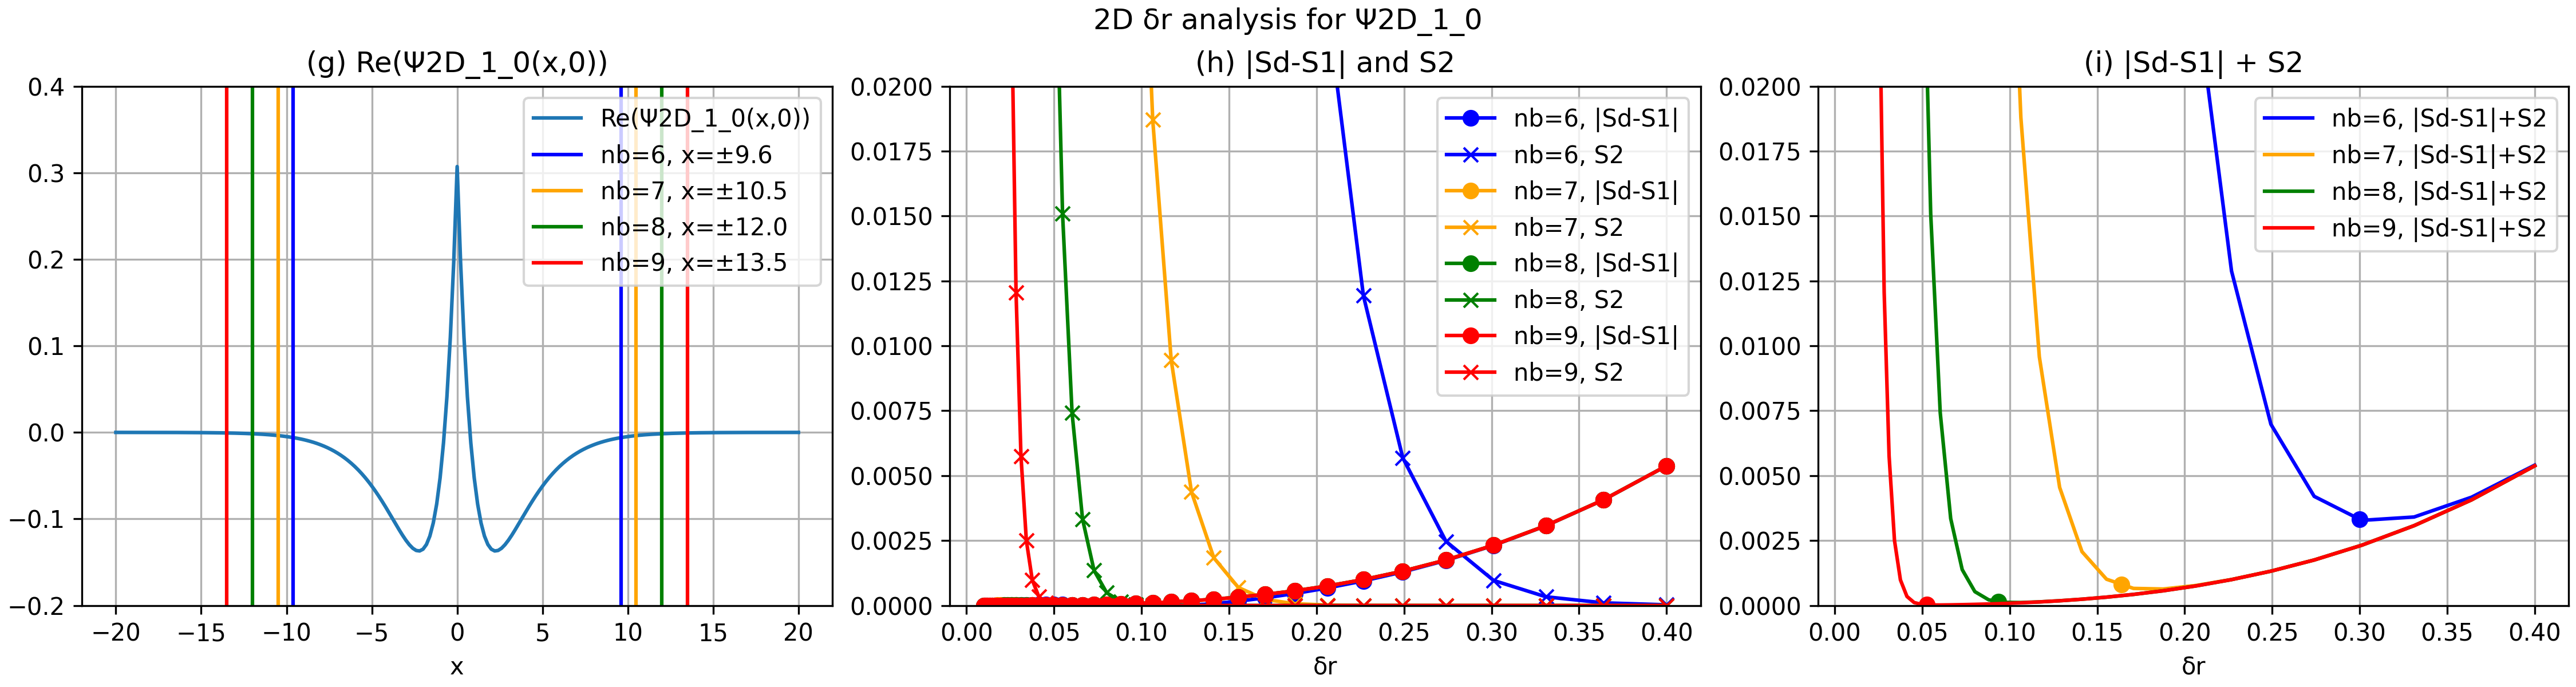
\includegraphics[width=\columnwidth]{paper2025_figs/dq_tradeoff/eval2d_dq_geom_1_0.png}
        \caption{2次元モデル $\PsiTwoD_{1,0}$}
        \label{subfig:dq-tradeoff-2d-1-0}
    \end{subfigure}
    \caption{いくつかの $\nb$ における$|\Sd-S_1|$と$S_2$の関係}
    \label{fig:dq-tradeoff}
    \begin{flushleft}\small 
        
        (a) は1次元モデル $\PsiOneD_1$、(b) と (c) はそれぞ
        れ2次元モデルの $\PsiTwoD_{0,0}$ と $\PsiTwoD_{1,0}$ に対する評価結
        果。(A1)〜(C1) は波動関数の $y=0$ 切片における実部の値と、選択した
        $\deltar$ に対応する計算領域境界（$\pm L/2$）を示す。(A2)〜(C2) は離散化
        誤差とカットオフ誤差を個別にプロットしたものであり、(A3)〜(C3) はその和
        を示す。この誤差の和が最小となる点がトレードオフの均衡点であり、最適な
        $\deltar$ を与える。

    \end{flushleft}
\end{figure}
\clearpage

\subsubsection{サンプリング定理に基づく時間刻みの条件}
\label{subsubsec:deltat-selection-results}

時間発展の期間を $t=1.0\ \mathrm{a.u.}$（物理時間で約 $24.19\ \mathrm{as}$）に固
定し、Suzuki-Trotter分割数 $\nT$ を変化させた際の誤差上限 $\BN{\gamma}(\psi;t)$
と、実際に観測されたシミュレーション誤差 $\xiN{\gamma}$ の関係を図
\ref{fig:trotter-error-t1-part1}および図\ref{fig:trotter-error-t1-part2}に示す
（$\gamma=1,2$ はTrotter次数）。なお、波動関数 $\PsiTwoD_{1,0}$ の時間発展周期が
$2\pi/E_2 \approx 28.27$ であることを考慮し、約1周期分に相当する $t=30$ での評価
結果については補助資料
\ref{smsec:parameter-selection-for-minimum-error-analysis-details}に譲る。

各グラフには、サンプリング定理に基づく $\nT$ の下限値である $\nTpminTwoD$ および
$\nTkminTwoD$ を垂直線で示している。縦軸はエネルギーではなく、式
\eqref{eq:observed-trotter-error-1st}および\eqref{eq:observed-trotter-error-2nd}
で定義した波動関数振幅の差のノルムである。

特筆すべきは、対象状態の量子数によるTrotter次数の効果の違いである。方位量子数
$m=0$ を持つ $\PsiTwoD_{0,0}$ および $\PsiTwoD_{1,0}$ の結果（図
\ref{subfig:trotter-error-2d-0-0-6b-t1}〜\ref{subfig:trotter-error-2d-1-0-9b-t1}）
では、Trotter次数 $\gamma$ の違いによる明確な精度の差は見られなかった。これ
は、Burgarthらが3次元水素原子モデルにおいて「方位量子数が0の固有関数ではTrotter
次数を上げても精度の改善は見られない」と報告した知見
\cite{Burgarth2024.PhysRevResearch.6.043155}と、次元は異なるものの一致する
結果である。

一方で、方位量子数 $m=1$ を持つ $\PsiTwoD_{1,1}$ の結果（図
\ref{subfig:trotter-error-2d-1-1-6b-t1}〜\ref{subfig:trotter-error-2d-1-1-9b-t1}）
では、分割数 $\nT$ が小さい領域において1次（$\xiN{1}$）と2次（$\xiN{2}$）の
Trotter分解の間に明確な精度差が確認できる。これは、角運動量を持つ状態においては
運動エネルギーとポテンシャルエネルギーの非可換性がより強く影響するため、高次分解
による誤差改善効果が顕著に現れたものと考えられる。

全体的な傾向として、いずれの条件でも分割数 $\nT$ の増加に伴い誤差 $\xiN{1},
\xiN{2}$ は減少するが、運動エネルギー項に対するサンプリング定理の下限値 $\nT =
\nTkminTwoD$ の付近で減少が飽和する。$\PsiTwoD_{1,1}$ では $\nT > \nTkminTwoD$
の領域でもわずかな誤差の減少が見られるものの、実質的な影響は小さい。これは、この
領域に達すると時間誤差（Trotter誤差）よりも空間分解能に起因する空間離散化誤差
$\errdisc$ が支配的になるためである。

したがって、ここに示した条件下では、サンプリング定理から導かれる下限値
$\nTkminTwoD$ を大きく超える分割数を設定しても、計算コストが増大するだけで全体誤
差の改善には寄与しないと言える。空間誤差との関係については、例えば図
\ref{subfig:trotter-error-2d-0-0-6b-t1}（$\nb=6$）と図
\ref{subfig:trotter-error-2d-0-0-9b-t1}（$\nb=9$）を比較すると明確である。空間分
解能 $\nb$ を高めることで、Trotter誤差が飽和した後の残存誤差のフロア（底）が1/10
程度まで大きく縮小していることが確認できる。


\begin{figure}[ht]
    \centering
    \begin{subfigure}{0.45\columnwidth}
        \centering
        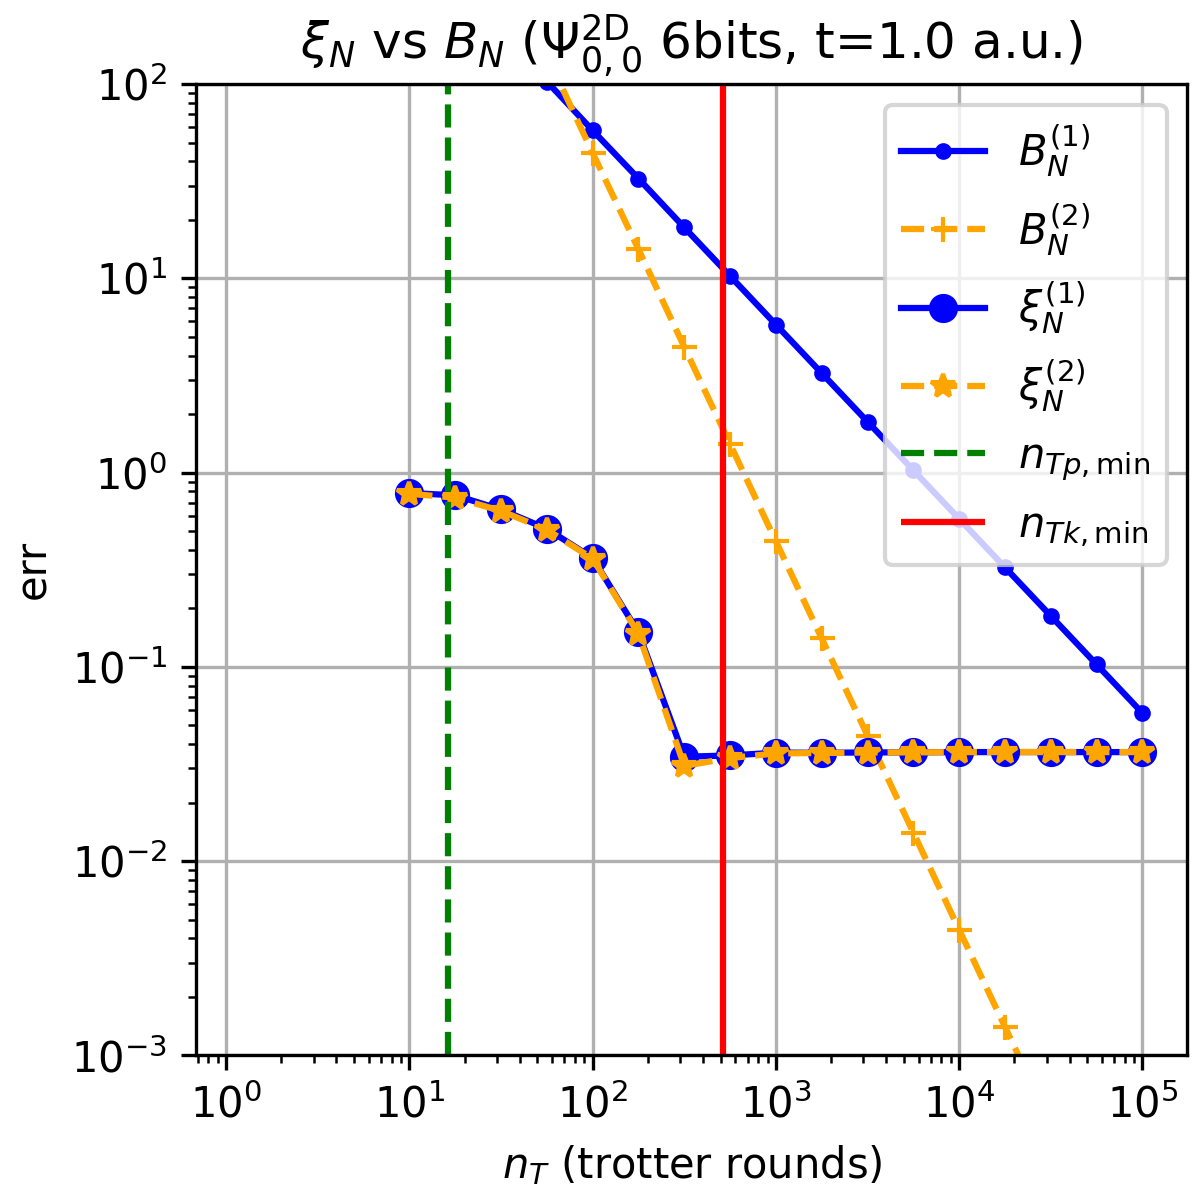
\includegraphics[width=1\columnwidth]{paper2025_figs/sdt_error/trotter_err_n0_m0_6b_t1.0.png}
        \caption{$\PsiTwoD_{0,0}, \nb=6, t=1.0$}
        \label{subfig:trotter-error-2d-0-0-6b-t1}
    \end{subfigure}
    \begin{subfigure}{0.45\columnwidth}
        \centering
        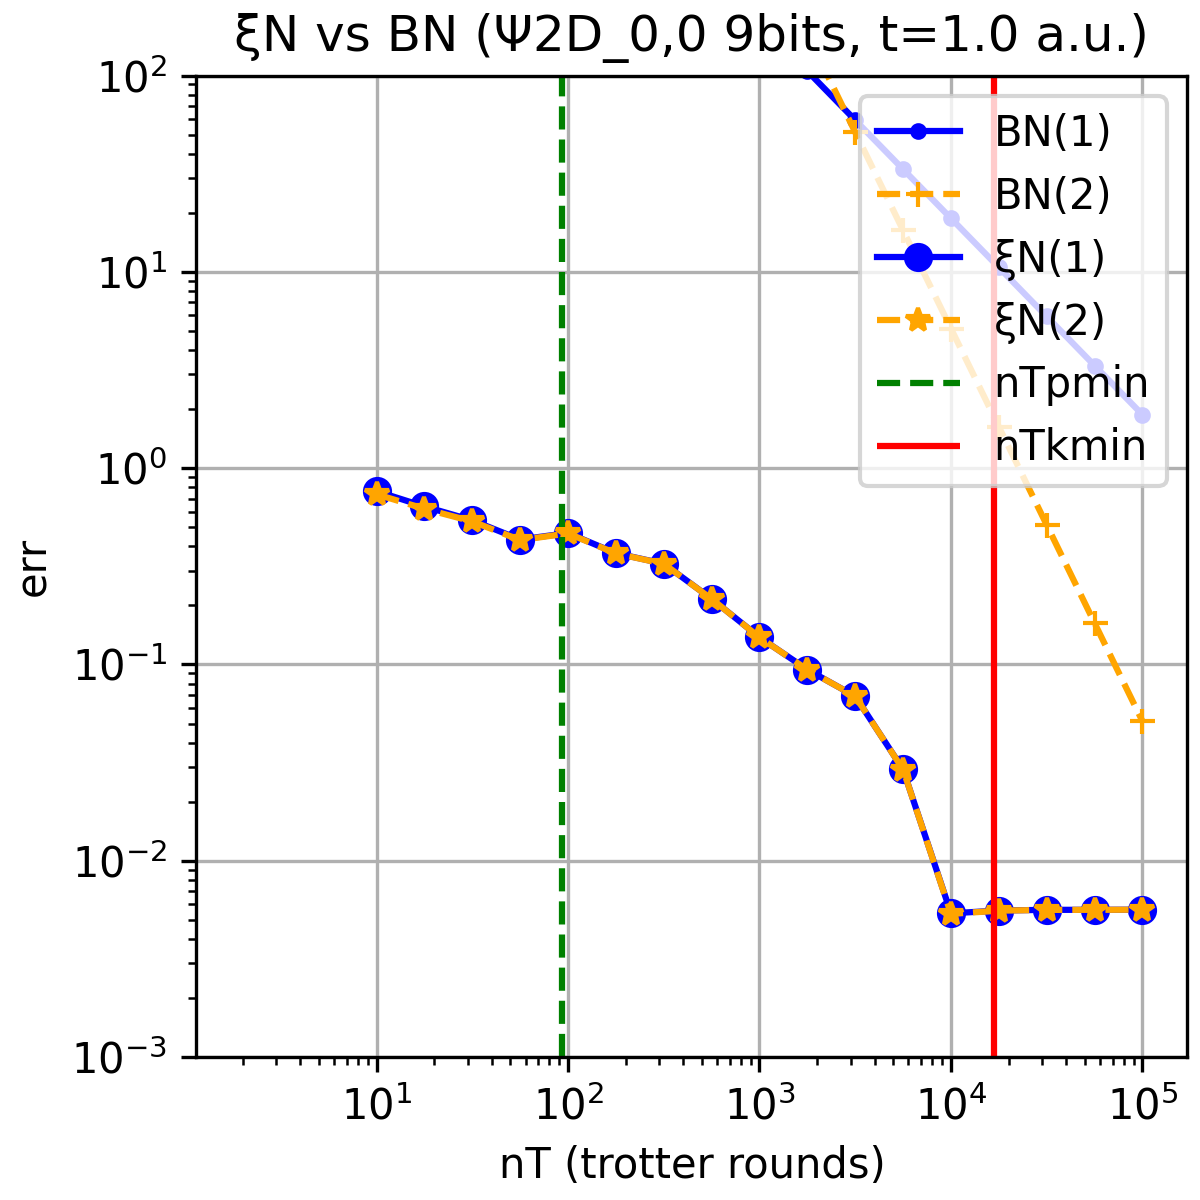
\includegraphics[width=1\columnwidth]{paper2025_figs/sdt_error/trotter_err_n0_m0_9b_t1.0.png}
        \caption{$\PsiTwoD_{0,0}, \nb=9, t=1.0$}
        \label{subfig:trotter-error-2d-0-0-9b-t1}
    \end{subfigure}

    \begin{subfigure}{0.45\columnwidth}
        \centering
        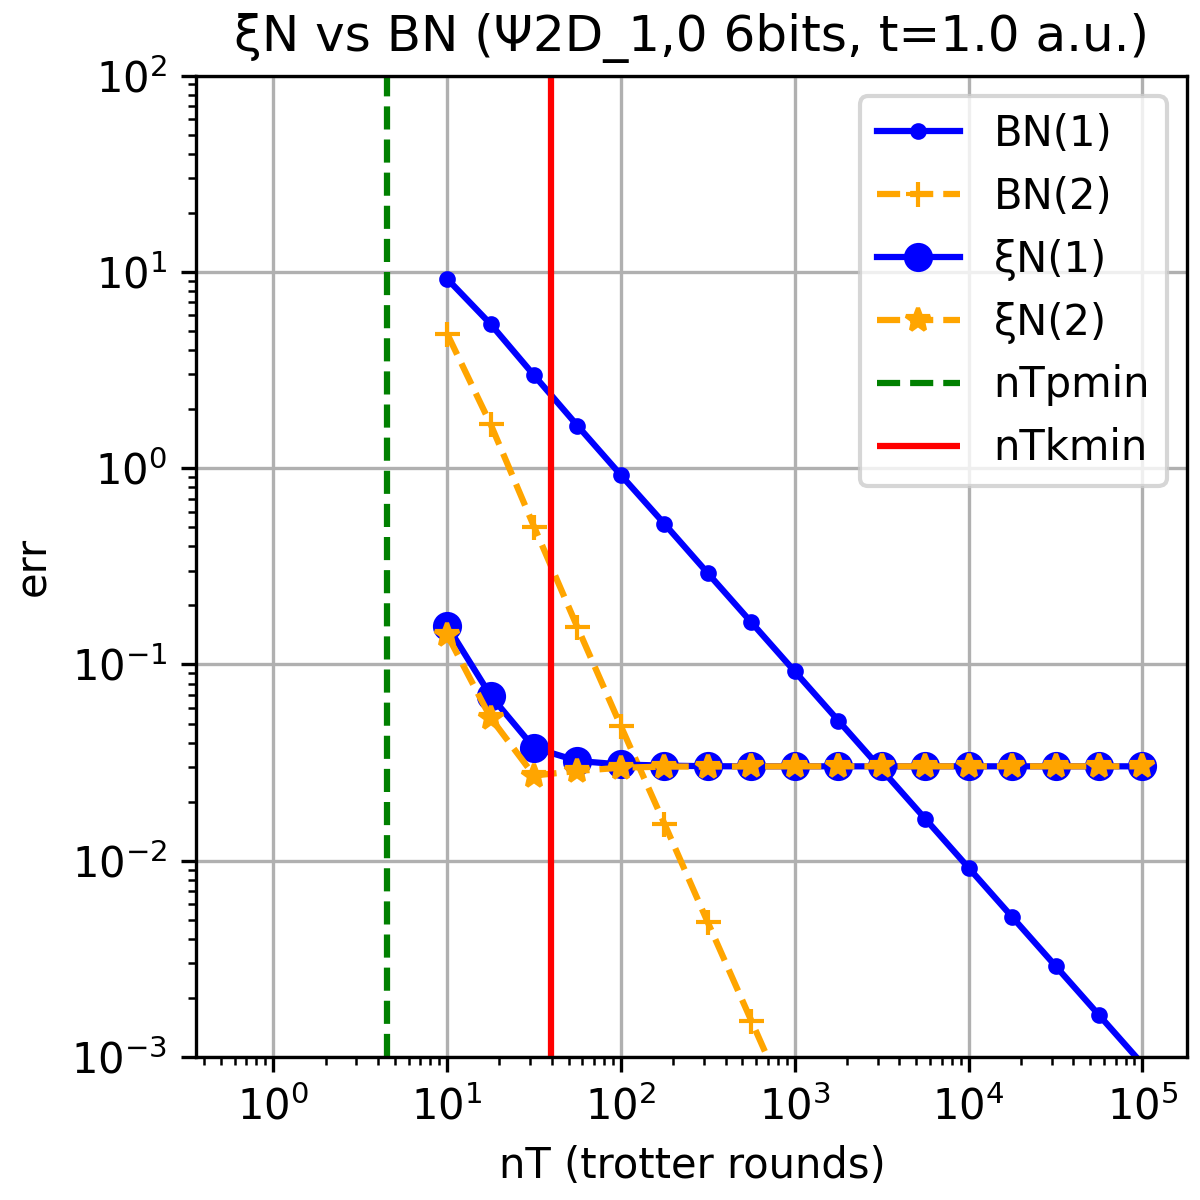
\includegraphics[width=1\columnwidth]{paper2025_figs/sdt_error/trotter_err_n1_m0_6b_t1.0.png}
        \caption{$\PsiTwoD_{1,0}, \nb=6, t=1.0$}
        \label{subfig:trotter-error-2d-1-0-6b-t1}
    \end{subfigure}
    \begin{subfigure}{0.45\columnwidth}
        \centering
        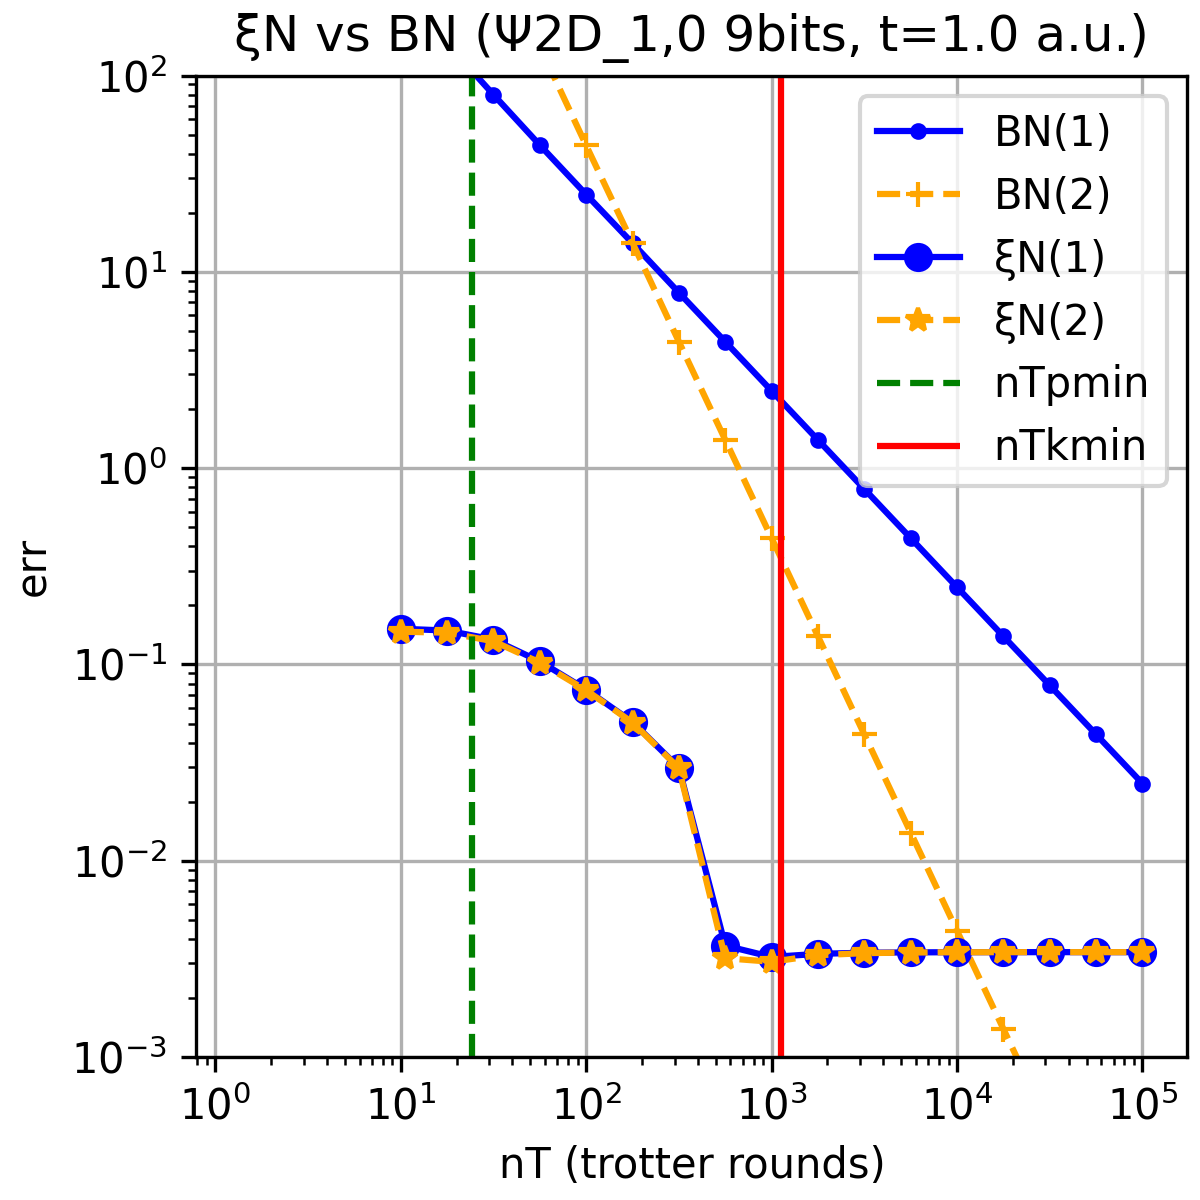
\includegraphics[width=1\columnwidth]{paper2025_figs/sdt_error/trotter_err_n1_m0_9b_t1.0.png}
        \caption{$\PsiTwoD_{1,0}, \nb=9, t=1.0$}
        \label{subfig:trotter-error-2d-1-0-9b-t1}
    \end{subfigure}

    \caption{時間発展期間$t=1.0$ での分割数$\nT$に対する誤差の上限 $\BN{\gamma}$ と観測値 $\xiN{\gamma}$}
    \label{fig:trotter-error-t1-part1}
    \begin{flushleft}\small
        2次元モデルにおけるTrotter分割数と誤差の関係。時間発展期間は $t=1.0$ 固
        定。$\xiN{1}, \xiN{2}$ はそれぞれ1次、2次のTrotter分解による全観測誤差
        （空間誤差等も含む）。$\BN{1}, \BN{2}$ は解析的に求めたTrotter誤差の理論
        的上限値である。垂直線 $\nT=\nTpminTwoD$ および $\nT=\nTkminTwoD$ は、サ
        ンプリング定理の要請から定まるポテンシャル項および運動エネルギー項に対す
        る分割数の理論的下限値を示す。
    \end{flushleft}
\end{figure}

\begin{figure}[ht]
    \centering
    \begin{subfigure}{0.45\columnwidth}
        \centering
        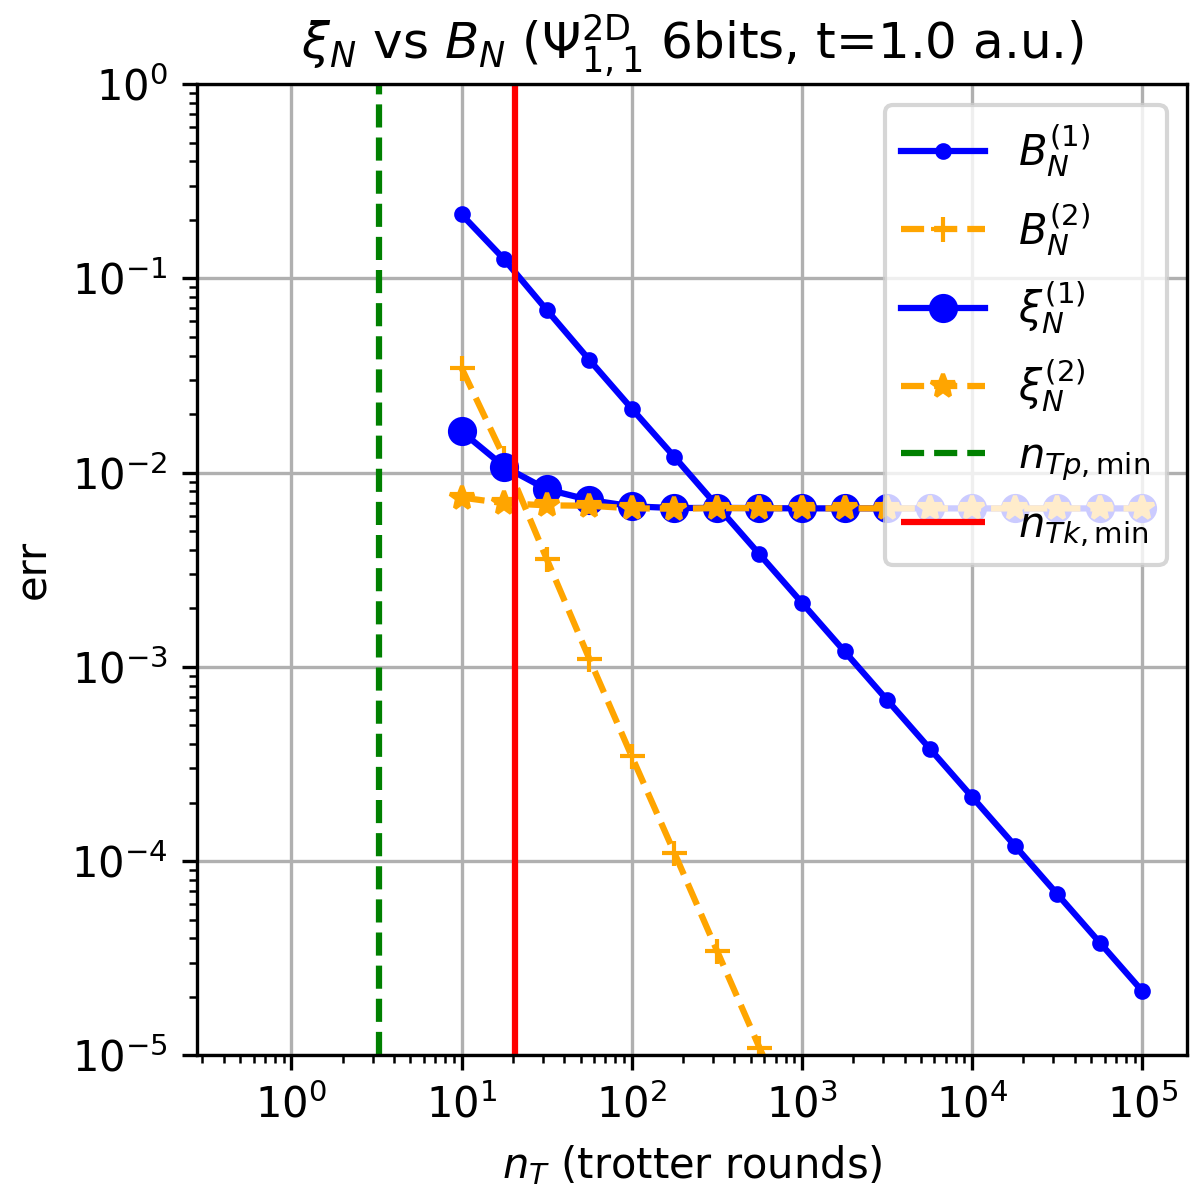
\includegraphics[width=1\columnwidth]{paper2025_figs/sdt_error/trotter_err_n1_m1_6b_t1.0.png}
        \caption{$\PsiTwoD_{1,1}, \nb=6, t=1.0$}
        \label{subfig:trotter-error-2d-1-1-6b-t1}
    \end{subfigure}
    \begin{subfigure}{0.45\columnwidth}
        \centering
        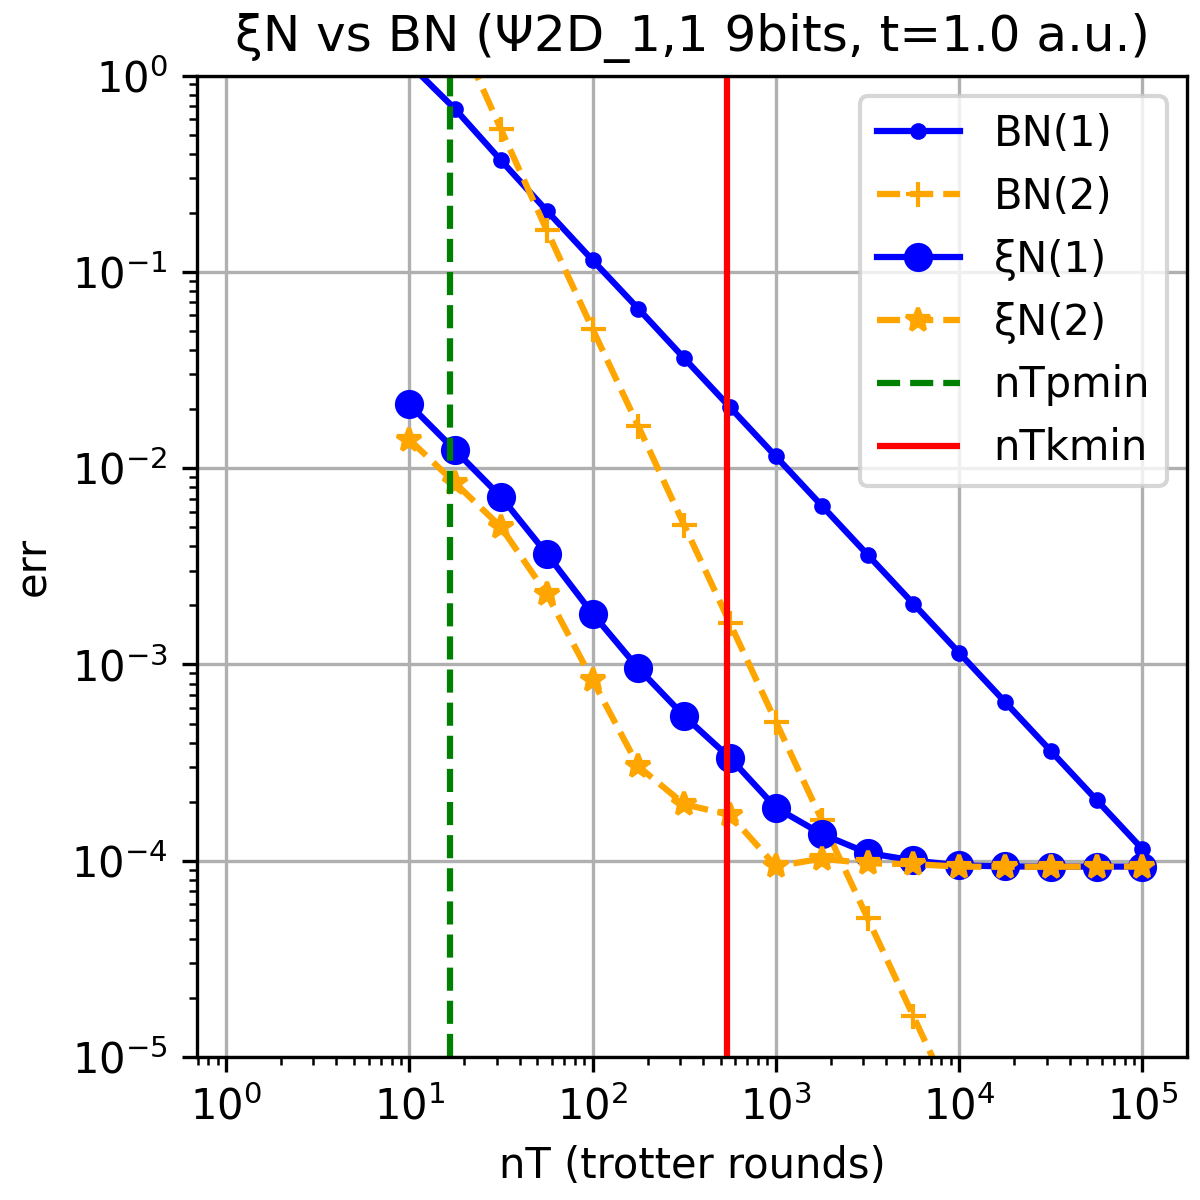
\includegraphics[width=1\columnwidth]{paper2025_figs/sdt_error/trotter_err_n1_m1_9b_t1.0.png}
        \caption{$\PsiTwoD_{1,1}, \nb=9, t=1.0$}
        \label{subfig:trotter-error-2d-1-1-9b-t1}
    \end{subfigure}
    \caption{時間発展期間 $t=1.0$ における分割数 $\nT$ に対する誤差の上限 $\BN{\gamma}$ と観測値 $\xiN{\gamma}$（続き）}
    \label{fig:trotter-error-t1-part2}
    \begin{flushleft}\small
        方位量子数 $m=1$ を持つ波動関数 $\PsiTwoD_{1,1}$ に対する評価結果。$\nT$
        が小さい領域において、1次と2次のTrotter分解による精度の差が顕著に表れて
        いる。
    \end{flushleft}
\end{figure}

\clearpage
\end{document}
